\documentclass[a4paper]{article}

\usepackage{microtype}
\usepackage{fullpage}
\usepackage{mathtools}
\usepackage{amsfonts}
\usepackage{tikz}
\usepackage{pgfplots}
\usepackage{hyperref}
\usepackage{amsthm}
\usepackage{xcolor}
\usepackage[noabbrev,nameinlink]{cleveref}
\usepackage{caption}
\usepackage{subcaption}
\usepackage{setspace}
\usepackage[backend=biber,style=authoryear,maxbibnames=99,hyperref=true]{biblatex}

\setstretch{1.15}

\addbibresource{src/paper/references.bib}

\usepgfplotslibrary{fillbetween}
\usetikzlibrary{shapes}
\pgfplotsset{compat=1.17}

\newtheorem{theorem}{Theorem}
\newtheorem{proposition}{Proposition}
\newtheorem{corollary}{Corollary}
\newtheorem{lemma}{Lemma}
\newtheorem{assumption}{Assumption}

\newcommand{\dt}{\mathrm{d}t}
\newcommand{\ds}{\mathrm{d}s}
\newcommand{\di}{\mathrm{d}i}
\newcommand{\dG}{\mathrm{d}G}
\newcommand{\E}{\mathbb{E}}
\newcommand{\Var}{\mathrm{Var}}

\DeclarePairedDelimiter\floor{\lfloor}{\rfloor}

\title{The value of being indispensable: a cooperative approach to bargaining with a continuum of players}
\author{Martin Stancsics}

\begin{document}

\maketitle

\begin{abstract}
    This paper investigates the idea of using concepts random order values, a concept from cooperative game theory, to model bargaining outcomes in games with an indispensable player and a continuum of fringe players.
    I show that this approach proves to be very tractable in a number of settings, and leads to results that are in line with one's intuitive expectations about bargaining outcomes.
    Thus, it can be a useful tool in modelling situations where one does not want to attribute all the bargaining power to one type of market participants, and at the same time would like to avoid having to deal with an explicit multi-stage bargaining game.
    On one hand, this paper provides a taxonomy of the various results found in some applied papers.
    Furthermore, it introduces some new results pertaining to the case of multiple types of fringe players.
    The utility of this approach is demonstrated via a simple model of two-sided markets.
    The results in this paper are intended to be used as a tool-kit for embedding bargaining outcomes into more complex models.
\end{abstract}


\section{Motivation}

Using cooperative game theory to model bargaining outcomes in a tractable way has quite a few examples in the industrial organization literature.
This is in part motivated by the appealing properties of the resulting gain distributions, their tractability, but also by the long line of theoretical studies showing that various bargaining procedures lead to such outcomes.
For example, \textcite{gul1989bargaining,winter1994demand,hart1996bargaining,inderst2003bargaining,} or, perhaps most relevant to this paper, \textcite{stole1996intra} all propose various extensive-form bargaining games in which the expected outcomes correspond to players' Shapley-values.

In terms of applications, the case of one indispensable player and a large number of small ones is particularly important in a number of settings.
Examples include intra-firm ownership strutures \parencite{hart1990property}, wage bargaining \parencite{stole1996intra,stole1996organizational,levy1997individual}, collusion and mergers \parencite{segal2003collusion} and upstream-downstream supply chains \parencite{inderst2003bargaining,montez2007downstream}.
The study of multi-sided markets (paltforms) is also a good fit for this modeling approach, as the platform is often indispensable for the fringe firms, but the latter are also numerous enough to be approximated by a continuum.\footnote{
    \textcite{huang2022shapley} is one of the very few examples of using cooperative game theory in this setting.
}

A common feature of most of the aforementioned papers is that they assume a finite number of players.
However, as is often the case in economics, infinite-player approximations turn out to be more tractable while retaining the main conclusions of the finite models from which they arise.
Perhaps most importantly, the resulting profit shares become continuous and differentiable functions of the size of the fringe, which is particularly useful when embedding these results into more complex models.

Cooperative games with a finite number of atomic players and a continuum of non-atomic ones are called mixed or oceanic games \parencite{milnor1978values}, and have been studied in the literature of cooperative game theory.
Most papers in this line of research focus on questions such as for which games the Shapley-value exists and is unique \parencite{hart1973values}, and whether various approaches (namely, characterizing the value using a set of axioms, and taking the limit of the value of finite-player games) lead to the same result \parencite{fogelman1980asymptotic}.\footnote{
    \textcite{hart1973values} shows that in the case of mixed games, the usual axioms do not characterize a unique value in general.
    However, \textcite{fogelman1980asymptotic} demonstrates that, for a quite general subset of games, the asymptotic approach leads to one specific element from the set characterized by the axiomatic approach. 
}
My aim with this paper is both more general and more specific in certain aspects.
For one, I am only interested in the asymptotic approach, and withing that, a specific series of finite games.
Furthermore, I restrict my attention to one specific type of games, namely those with an indispensable player, and a continuum of fringe players consisting of a finite number of types.
This in turn allows me to go beyond the usual Shapley-value, and obtain results for a more general set of solution concepts: random order values.
In the case of multiple types of fringe players, I also present a number of new results for the Shapley value and the weighted value.
In particular, I derive the value of the different types of fringe players in the multi-sided setting, and demonstrate how they are related to their marginal contributions.
Additionally, due to having more structure in the model, I am able to provide more concrete results, investigate some comparative statics, as well.

Despite their theoretical appeal and their tractability, oceanic games saw very little use in the industrial organization, and, more generally, applied economics literature.
The most prominent examples are \textcite{stole1996intra, stole1996organizational} and \textcite{levy1997individual}, all of which use the Shapley-value to model wage bargaining, and consider the case of divisible labor (continuum of workers).
The first two of these paper also provides microfoundations for the Shapley value and the weighted value in the intra-firm bargaining setting.
To showcase the utility of this approach, I also build a simple model of two-sided markets.
In addition to the aformentioned papers, this model includes two new features: (1) results about the distribution of the value between the various types of fringe players, and (2) using the weighted value in a multi-sided setting.

In the following sections, I propose an oceanic game with the main feature that the large player is indispensable for creating value.\footnote{
    This assumption will be somewhat relaxed throughout some of the generalizations.
}
Such a model applies to all the settings mentioned above, such as intra-firm bargaining, vertical supply chains, or multi-sided markets.
I demonstrate that the random order values of the players in those models are described by very tractable expressions that have nice geometric interpretations.
Additionally, the outcomes are in line with one's intuitive expectations of bargaining power in such situations.
Finally, I demonstrate the usefulness of this approach by building a simple model of two-sided markets, where the various players' shares are determined by their (weighted) Shapley values.


\section{One-sided case}

In this section I examine the case of identical fringe players.
Many of these results are known in the literature, but I include them here for three reasons.
First, to provide build intuition for the more general case later on.
Second, to highlight the similarities to the multi-sided case, and to provide a bridge between the two.
Finally, I also express the fringe's value in terms of its weighted marginal contributions, which is a useful result in its own right.
In the main text, I only consider the most straightforward case (one large completely indispensable player), but in \ref{sec:extensions} I will somewhat relax these assumptions.

Let us start by defining the cooperative game that describes this situation.
Consider a game with two types of players: a major player $P$ and $n$ smaller players $A_i$, $1 \leq i \leq n$.
Formally, let us denote the set of all players as $N = \{P, A_1, \dots, A_n\}$.
Assume that (1) no coalition of players can achieve a positive value without the participation of $P$ and (2) players $A_i$ are identical to each other.
Let $n_T(S)$ denote the number of players of type $T \in \{P, A\}$ in coalition $S$.
Under these assumptions, the characteristic function of this game (the value that a coalition $S \subset N$ can achieve) is the following:
\begin{align*}
    v(S) = \begin{cases}
        0                              & \text{if } P \notin S \\
        f\left(\frac{n_A(S)}{n}\right) & \text{otherwise}.
    \end{cases}
\end{align*}
Such a game can represent, for example, a (one-sided) platform and a number of potential entrants, where the entrants can only reach their prospective consumers through the platform, or as a vertical supply chain with one upstream producer and a number of downstream sellers.

Before delving into the various values, let us characterize the conditions under which this game is monotone and superadditive.
Monotonicity requires that the value of any coalition is weakly higher than the value of any of its subsets.
Superadditivity on the other hand requires that the value of the union of two disjoint coalitions is weakly higher than the sum of their values.
The latter is a key property of cooperative games, as it ensures that it always pays off to form the grand coalition (i.e., the coalition that includes all players).
Furthermore, in the context of bargaining, these properties provide some theoretical support for using the Shapley-value or the weighted value to represent bargaining outcomes, as many results creating a link between non-cooperative bargaining games and the values of cooperative games often rely on these assumptions.\footnote{
    For example, the results in \textcite{gul1989bargaining} rely on superadditivity, while monotonicity suffices for \textcite[]{hart1996bargaining}.
}
In this specific setting, characterizing monotonicity and superadditivity is extremely straightforward.
\begin{proposition}
    \label{prop:monotone}
    The game $(N, v)$ is monotone and superadditive if and only if $f$ is increasing and $f(0) \geq 0$.
\end{proposition}
The intuition behind this result is quite straightforward.
As player $P$ is necessary to create any value, no two disjoint coalitions can both achieve a positive value.
Therefore, superadditivity is equivalent to monotonicity in this case.

In the following, let us assume that the assumptions required for monotonicity are always satisfied (i.e., $f$ is monotone increasing).\footnote{
    This assumption is not entirely innocuous.
    For example, having more small firms could in theory lead to stronger competition, decreasing total profits.
    However, it often holds in models with network effects \parencite{rochet2003platform} or with consumers having taste for variety \parencite{anderson2020aggregative}.
}
As a side note, it also ensures that the game is of bounded variation, and thus the main theorem in \textcite{fogelman1980asymptotic} applies.
Namely, the asymptotic and the axiomatic approach of characterizing the Shapley-value of the game both lead to the same result\footnote{
    More precisely, the asymptotic value coincides with the axiomatic one derived using the uniform distribution.
    For a more detailed discussion, see \textcite{fogelman1980asymptotic}.
}.
This result could also be used to prove \cref{prop:one_sided} instead of the direct proof provided in \cref{sec:proofs}.

\subsection{Random order values}

Random order values are a class of cooperative solution concepts characterized by efficiency, monotonicity, linearity and the null-player axiom \parencite{weber1988probabilistic}.
That is, they are a generalization of the Shapley value, where the axiom of symmetry is relaxed.
Another way to think about them is that they are the average marginal contribution of a player to all possible coalitions, where the average is taken according to some probability distribution over the permutations of the players.

In this specific game, a random order value can be obtained in the following way.
First, take all permutations of the players, and assign a probability to each permutation.
Then, the random order value of player $P$ is the expected marginal contribution of $P$ to the value of the coalition preceding it, where the expectation is taken according to said probability distribution.

For the remainder of the paper, let us use the following notation: $\varphi_P^n$ denotes the (depending on section, Shapley, weighted or random order) value of player $P$ in the game with players $N = \{P, A_1, \dots, A_n\}$.
Then, formally,
\begin{align*}
    \varphi_P^n = \frac{1}{(n+1)!} \sum_{R} \Pr(R) [ v(\mathcal{P}_P^R \cup \{i\}) - v(\mathcal{P}_P^R) ]
\end{align*}
where $R$ is a permutation of all players, and $\mathcal{P}_P^R$ is the set of players before $P$ in the permutation $R$. \footnote{
    For example, if $R = \{A_1, P, A_2\}$, then $\mathcal{P}_P^R = \{A_1\}$.
}

Random order values are of interest for a number of reasons.
First, they are a natural extension to the Shapley value and the weighted value.
Furthermore, they provide a convenient framework, of which all subsequent results (Shapley value, weighted value, multiple big players) are special cases.

Utilizing the fact that the value of any coalition is zero without $P$, and that -- conditional on player $P$ being in a coalition -- a coalition's value only depends on the number of fringe firms in it, the above expression can be simplified to the following:
\begin{align*}
    \varphi_P^n = \frac{1}{n+1} \sum_{k=0}^n \Pr(|\mathcal{P}_P| = k) f(k/n),
\end{align*}
where $\Pr(|\mathcal{P}_P| = k)$ is determined by the probability distribution over the permutations.

Now let us look at the asymptotic limit of this expression, as the number of fringe players goes to infinity.
The following proposition demonstrates the main idea of this paper: even as the number of fringe players goes to infinity, the value of the big player does not converge to the worth of the grand coalition, $f(1)$.
Or, in other words, the fringe, even when its members are infinitesimally small, still retains some bargaining power.
As a corollary, the continuous fringe model can be thought of as a more tractable approximation of bargaining between a finite number of fringe players, as it retains the latter's main features.

\begin{proposition}
    \label{prop:one_sided_general}
    Let $f$ be continuous on [0, 1]. Furthermore, let us denote the random variable $\frac{|\mathcal{P}_P|}{n}$ as $X_n$. Assume that $X_n \xrightarrow[]{d} X$ with cdf $G_X(t)$ and (if exists) pdf $g(t)$.
    Then
    \begin{align*}
        \varphi_P^\infty = \lim_{n \to \infty} \varphi_P^n = \int_0^1 f(t) \dG(t) = \int_0^1 g(t) f(t) \dt,
    \end{align*}
    with the last equality holding if $X$ is a continuous random variable.
\end{proposition}

Now let us turn to the value of the fringe.
The following corollary shows that the aggregated value of the fringe remains positive even in the limit.
In other words, even though the fringe players become smaller and more numerous, they do not lose all of their bargaining power, and still end up with a positive payoff in the end.
\begin{corollary}
    \label{cor:fringe_value_general}
    The aggregated value of the fringe is
    \begin{align*}
        \varphi_A^\infty = f(1) - \int_0^1 f(t) \dG(t).
    \end{align*}
    Furthermore, if $f$ is differentiable on $[0, 1]$, then the value of the fringe can also be expressed as
    \begin{align*}
        \varphi_A^\infty = \int_0^1 G(t) f'(t) \dt.
    \end{align*}
\end{corollary}

It also provides us with two ways of thinking about the value of the fringe.
First, due to random order values being efficient, it can be thought of as the leftover from the total value after subtracting the value of the big player.
Alternatively, as the second part of the corollary demonstrates, it is also related to the marginal contributions of the fringe agents.
The only difference from the big player's value is that we have to multiply these marginal contributions by the probability of the big player appearing before the fringe firm in question, as otherwise they would be zero.
The latter interpretation will be particularly useful when thinking about the value of the fringe in the multi-sided setting.

It also follows immediately from the previous proposition that (for a fixed total pie size $f(1)$) player $P$ gets a larger share when $f(t)$ is larger for every $t$.
That is, when only a relatively small fraction of the fringe is needed to create a large part of the total potential surplus (e.g. fringe players' products are substitutes of each other), then player $P$ is able to appropriate a larger share of the total value.
This result aligns with our natural intuition that player $P$ has a better bargaining position in this case, than if only coalitions with most of the fringe firms on board could obtain high values.
In contrast, when fringe players are more complementary to each other, the big player can only obtain a smaller share, as its bargaining power is more limited.


\subsection{Shapley value}

Now let us turn our attention to an important special case of random order values: the Shapley value.
It can be characterized by being the random order value that additionally also satisfies the axiom of symmetry.
This axiom requires that if two players are identical in terms of the characteristic function, then they should receive the same value.
Equivalently, it is the same as requiring that all permutations have an equal probability.

The following proposition and corollary derives the limit of the Shapley value for the big player and the fringe, respectively.

\begin{proposition}
    \label{prop:one_sided}
    Let $f$ be continuous on [0, 1]. Then
    \begin{align*}
        \varphi_P^\infty = \lim_{n \to \infty} \varphi_P^n = \int_0^1 f(t) \dt .
    \end{align*}
\end{proposition}

\begin{corollary}
    \label{cor:fringe_value}
    The aggregated Shapley-value of the fringe is
    \begin{align*}
        \varphi_A^\infty = f(1) - \int_0^1 f(t) \dt.
    \end{align*}
    Furthermore, if $f$ is differentiable on $[0, 1]$, then the value of the fringe can also be expressed as
    \begin{align*}
        \varphi_A^\infty = \int_0^1 t f'(t) \dt.
    \end{align*}
\end{corollary}

Because the Shapley value is a special case of the random order value, these results are quite straightforward consequences of \cref{prop:one_sided_general} and \cref{cor:fringe_value_general}.
One only has to notice that each permutation having an equal probability implies that the number of firms coming before $P$ is uniformly distributed on $1, \dots, n$, and thus the share of firms before $P$ converges in distribution to the uniform distribution on $[0, 1]$.
Alternatively, a more direct proof is provided in \cref{sec:proofs}, or a probabilistic justification can be found in \textcite{levy1997individual}.

The resulting Shapley values also have a nice geometric interpretation shown on \cref{fig:one_sided}.
Consider a rectangle with sides of length 1 and $f(1)$, respectively.
The grand coalition achieves the value $f(1)$, which is also the area of the rectangle.\footnote{
    Due to superadditivity, the grand coalition can be expected to form, and the main question is how the value is distributed between the big player and the fringe.
}
The value of the big player is then $\int_0^1 f(t) \dt$, which is simply the part of the rectangle below the graph of $f$, while the fringe gets the rest.
Thus, the graph of $f$ partitions the area (total value) into what the big player and the fringe can obtain.

\begin{figure}
    \centering
    \begin{subfigure}[b]{0.45\textwidth}
        \centering
        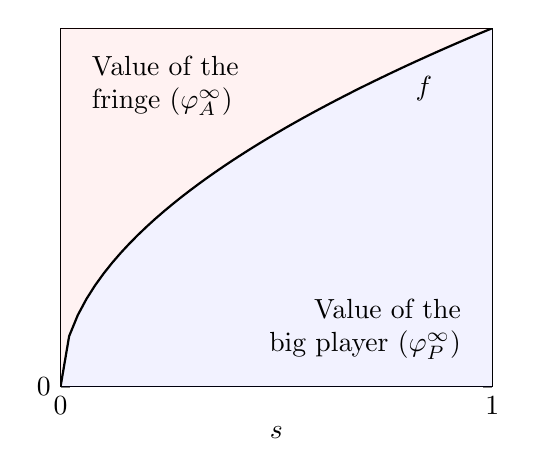
\begin{tikzpicture}[scale=0.8]
            \begin{axis}[xmin=0, xmax=1, ymin=0, ymax=1, samples at={0, 0.02, ..., 0.98, 1},
                    xtick={0, 1}, ytick={0}, xlabel={$s$}]
                \addplot[name path=f, thick] {x^0.5};
                \node[anchor=north west] at (axis cs: .8, .8^0.5) {$f$};
                \path[name path=bottom] (axis cs:0,0) -- (axis cs:1,0);
                \path[name path=top] (axis cs:0,1) -- (axis cs:1,1);

                \addplot [fill=blue, fill opacity=0.05] fill between [of=f and bottom];
                \addplot [fill=red, fill opacity=0.05] fill between [of=f and top];

                \node[anchor=north west, align=left] at (axis cs: .05, .95) {Value of the \\ fringe ($\varphi_A^\infty$)};
                \node[anchor=south east, align=right] at (axis cs: .95, .05) {Value of the \\ big player ($\varphi_P^\infty$)};
            \end{axis}
        \end{tikzpicture}
        \caption{Fringe players are each other's substitutes}
    \end{subfigure}
    \begin{subfigure}[b]{0.45\textwidth}
        \centering
        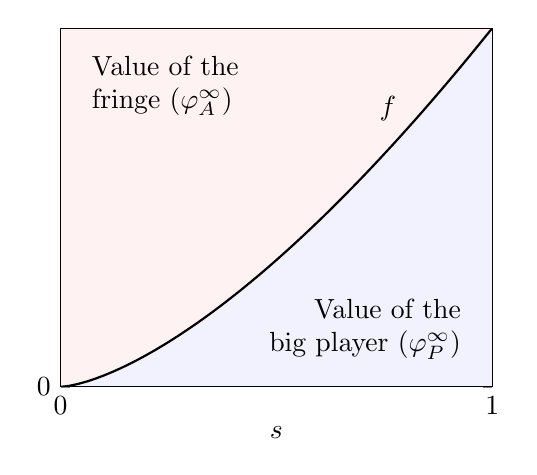
\begin{tikzpicture}[scale=0.8]
            \begin{axis}[xmin=0, xmax=1, ymin=0, ymax=1, samples at={0, 0.02, ..., 0.98, 1},
                    xtick={0, 1}, ytick={0}, xlabel={$s$}]
                \addplot[name path=f, thick] {x^1.5};
                \node[anchor=south east] at (axis cs: .8, .8^1.5) {$f$};
                \path[name path=bottom] (axis cs:0,0) -- (axis cs:1,0);
                \path[name path=top] (axis cs:0,1) -- (axis cs:1,1);

                \addplot [fill=blue, fill opacity=0.05] fill between [of=f and bottom];
                \addplot [fill=red, fill opacity=0.05] fill between [of=f and top];

                \node[anchor=north west, align=left] at (axis cs: .05, .95) {Value of the \\ fringe ($\varphi_A^\infty$)};
                \node[anchor=south east, align=right] at (axis cs: .95, .05) {Value of the \\ big player ($\varphi_P^\infty$)};
            \end{axis}
        \end{tikzpicture}
        \caption{Fringe players are each other's complements}
    \end{subfigure}
    \caption{Distribution of value between player $P$ (red) and the fringe (blue)}
    \label{fig:one_sided}
\end{figure}

Finally, the following corollary highlights that, even though the individual share of each $A_i$ vanishes as their number goes to infinity, their total value still remains positive.
\begin{corollary}
    \label{cor:fringe_value_2}
    $\varphi_P^\infty < f(1)$ and $\varphi_A^\infty > 0$ for any $f$ that is not constant.
\end{corollary}


\paragraph{Example: power function.}
\label{sec:power_function_example}

Let us illustrate the results of this section with a simple example.
Consider the case when $f(n) = n^\alpha$, for some $\alpha > 0$.
Assume that the bargaining takes place between player $P$ and a measure $\bar{n}$ of fringe players.
Thus, the value that the grand coalition can achieve is $\bar{n}^\alpha$.

\Cref{prop:many_sided_shapley} shows that the value of player $P$ in this case is
\begin{align*}
    \varphi_P^\infty(\bar{n}) = \int_0^1 (s \bar{n})^\alpha = \frac{1}{\alpha + 1} \bar{n}^\alpha,
\end{align*}
while the fringe gets the rest, i.e.,
\begin{align*}
    \varphi_A^\infty(\bar{n}) = \bar{n}^\alpha - \frac{1}{\alpha + 1} \bar{n}^\alpha = \frac{\alpha}{\alpha + 1} \bar{n}^\alpha.
\end{align*}

In words, regardless of the value of $\bar{n}$, the two types of players share the total value in the same proportion.
This proportion depends on the parameter $\alpha$ (\cref{fig:power_function_example}), which can be interpreted as the degree of substitutability between the fringe players.
More specifically, the higher $\alpha$ is, the more complementary the fringe players are to each other, and the larger the share they obtain.
In the limit, when $\alpha \to \infty$, the fringe obtains all the value, as essentially all players become indispensable, and share the total value equally.
On the other hand, when $\alpha \to 0$, the big players can appropriate all the value.

\begin{figure}
    \centering
    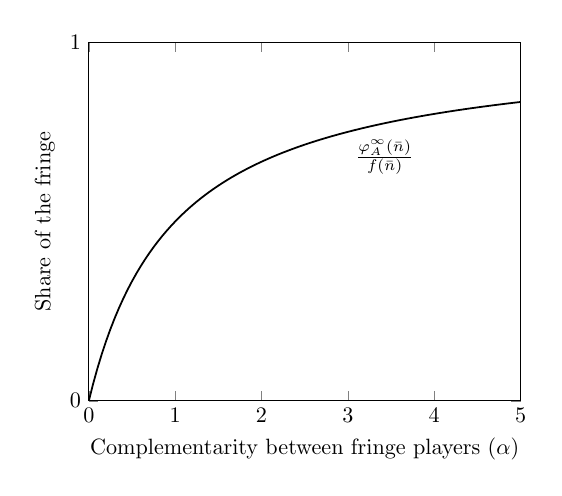
\begin{tikzpicture}[scale=0.8]
        \begin{axis}[xmin=0, xmax=5, ymin=0, ymax=1, samples at={0, 0.05, ..., 4.95, 5},
                xtick={0, 1, 2, 3, 4, 5}, ytick={0, 1},
                xlabel={Complementarity between fringe players ($\alpha$)}, ylabel={Share of the fringe}]
            \addplot[name path=f, thick] {x / (1 + x)};
            \node[anchor=north west] at (axis cs: 3, 3/4) {$\frac{\varphi_A^\infty(\bar{n})}{f(\bar{n})}$};
            \path[name path=bottom] (axis cs:0,0) -- (axis cs:1,0);
            \path[name path=top] (axis cs:0,1) -- (axis cs:1,1);
        \end{axis}
    \end{tikzpicture}
    \caption{Example: share of the fringe as a function of $\alpha$ (degree of complementarity between fringe players)}
    \label{fig:power_function_example}
\end{figure}


\subsection{Weighted values}
\label{sec:weighted_one_sided}

This section investigates the case of players having different levels of innate bargaining power.
One way to model this is by using weighted values \parencite{shapley1953additive}, which are a generalization of the Shapley value.
They are also a non-symmetric generalization of the Shapley value, albeit with more structure than random order values.
The idea behind them is that, in addition to the set of players and the characteristic function, the game is also endowed with a weight system, which is a vector of non-negative numbers, one for each player.
These weights determine how the value of a coalition is distributed amongst its members in the case when they are all equally important for the coalition.
Then, relying on the linearity of the value, this distribution can be extended to the case when the players are not equally important.

These weights can be thought of as the measure of some innate bargaining power, not reflected in the value function.\footnote{
    Although, this interpretation is not always appropriate.
    As \textcite{owen1968communications} demonstrates, there are games where the weighted value is not monotone increasing in a player's weight.
}
Further support for this interpretation in certain games can be found in \textcite{hart1996bargaining}, demonstrating that in a certain alternating offer bargaining game, weights are related to the probability of each player making the offer.\footnote{
    For example, only one player having a positive value corresponds to them making take it or leave it offers.
}
Additionally, \textcite{stole1996intra} provides an alternative microfoundation for the weighted value in the case of non-binding contracts.

For my purposes, it is sufficient to deal with the case of simple weights.
I.e., assume that there is at most one player with zero weight.
For my main result, I make use of an alternative, computational characterization of the weighted values. 
\textcite{kalai1987weighted} demonstratesd that weighted values can be calculated by weighting the permutations by the probabilities arising from the following sequential ordering procedure.
Start with the set of all players.
Let the probability of player $i$ being the last amongst the set of remaining players $R$ be $\lambda_i / \sum_{j \in R} \lambda_j$.
Continue until all players are exhausted.
This yields a well-defined probability for each permutation of players.

Now let us turn to deriving the weighted value and its limit for the big player and the fringe in this specific game.
First, I propose a lemma that characterizes the distribution of the number of players before $P$ in the limit, and then use it to derive the weighted value of the big player and the fringe.
Consider the game described in the previous section, and let the weights of players of type $A$ and $P$ be 1 and $\lambda$, respectively.
Let $X_n$ be a random variable representing the number of players before $P$ when players are ordered according to the previously described procedure.
Then, the probability of player $P$ having at most $k$ players of type $A$ before themselves is simply
\begin{align}
    \label{eq:entry_distr_discrete}
    \Pr(X_n \leq k) = \prod_{j=k+1}^n \frac{j}{j + \lambda}.
\end{align}
The following lemma establishes the continuous analogue of this statement.
\begin{lemma}
    \label{lem:entry_distr}
     As $n \to \infty$, $X_n \xrightarrow[]{d} X$ with the cdf $G_X(t) = \lambda^t$.
     Consequently, the corresponding probability density function is $g(t) = \lambda t^{\lambda - 1}$.
\end{lemma}

Now we have everything we need to derive the weighted value of both types of players.
Having \cref{eq:entry_distr_discrete} and \cref{lem:entry_distr} allows us to invoke \cref{prop:one_sided_general} to obtain the following proposition.\footnote{
    \textcite{stole1996intra} also derive essentially the same expression for the equilibrium outcome of their bargaining game with unequal profit distribution, and assert that it is equal to the weighted value.
}

\begin{proposition}
    \label{prop:one_sided_weighted}
    Let $f(t)$ be continuous on $[0, 1]$. Then
    \begin{align*}
        \varphi_P(\lambda, \infty) = \int_0^1 g(t) f(t) \dt
    \end{align*}
    where $g(t) = \lambda t^{\lambda - 1}$.

    Furthermore,
    \begin{align*}
        \varphi_A(\lambda, \infty) &= 1 - \int_0^1 g(t) f(t) \dt \\
                                   &= \int_0^1 G(t) f'(t) \dt,
    \end{align*}
    where $G(t) = t^\lambda$.
\end{proposition}

As before, the value of the big player can still be expressed as an integral of the value function, while the value of the fringe can be expressed as an integral of the marginal contributions of the fringe players.
The only difference is that, as in the case of the general random order value, the integrands are weighted by some probability distribution.
Depending on the shape of this distribution, regions corresponding to different masses of fringe firms can be over or underweighted in this integral, leading to different values.
Contrary to \cref{prop:one_sided_general}, the probability distribution has a specific functional form, and is characterized by a single parameter, $\lambda$.
\Cref{fig:weigh_function} illustrates the weighting function for various values of $\lambda$.

\begin{figure}[ht]
    \centering
    \begin{subfigure}[b]{0.45\textwidth}
        \centering
        \begin{tikzpicture}[scale=0.8]
            \begin{axis}[xmin=0, xmax=1, ymin=0, ymax=3, samples at={0.02, 0.04, ..., 0.98, 1},
                xtick={0, 1}, ytick={0, 1, 2, 3}, axis lines=left, xlabel={$t$}, legend pos=south east]
                \addplot[thick] {0.5 * x ^ (-0.5)};
                \addplot[thick, dashed] {1};
                \addplot[thick, dotted] {1.5 * x ^ (0.5)};
            \end{axis}
        \end{tikzpicture}
        \caption{$g(t)$}
    \end{subfigure}
    \begin{subfigure}[b]{0.45\textwidth}
        \centering
        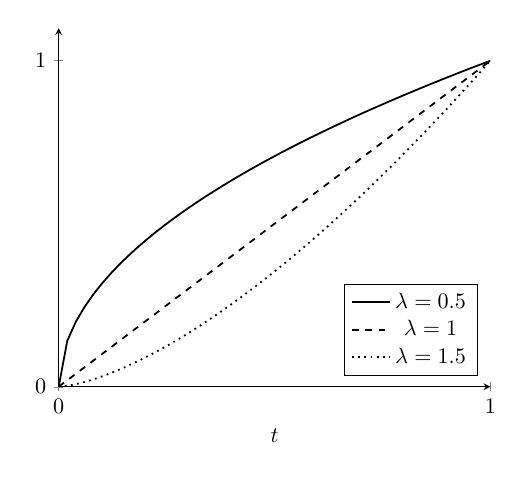
\begin{tikzpicture}[scale=0.8]
            \begin{axis}[xmin=0, xmax=1, ymin=0, ymax=1.1, samples at={0, 0.02, ..., 0.98, 1},
                xtick={0, 1}, ytick={0, 1}, axis lines=left, xlabel={$t$}, legend pos=south east]
                \addplot[thick] {x ^ (0.5)};
                \addplot[thick, dashed] {x};
                \addplot[thick, dotted] {x ^ (1.5)};
                \legend{$\lambda = 0.5$, $\lambda = 1$, $\lambda = 1.5$}
            \end{axis}
        \end{tikzpicture}
        \caption{$G(t)$}
    \end{subfigure}
    \caption{Illustration of the weighting function for various values of $\lambda$ in the weighted Shapley-value.}
    \label{fig:weigh_function}
\end{figure}

Now, let us examine how these weights impact the shares of the various players.
\begin{corollary}
    \label{cor:platform_value_weighted}
    $\varphi_P(\lambda, \infty)$ is increasing in $\lambda$ unless $f$ is constant.
\end{corollary}
It turns out, that a higher weight corresponds to a higher Shapley-value in this game.\footnote{
    This would not necessarily have to be the case, as demonstrated by \textcite{owen1968communications}.
},
supporting their interpretation as some kind of innate bargaining power.

Furthermore, the next corollary shows that the limit of the weighted value of $P$, as their weight goes to zero (infinity) is precisely the payoffs $P$ would achieve if $P$ were making (facing) take-it-or-leave-it offers.
\begin{corollary}
    \label{cor:paltform_value_weighted_2}
    If the weight of player $P$ goes to infinity (zero), its weighted Shapley value converges to $f(1)$ ($f(0)$).
\end{corollary}
This set of results highlights that utilizing (weighted) Shapley values to model bargaining outcomes provides an intermediate solution between inscribing all the bargaining power to one or the other player, and thus a generalization of take-it-or-leave-it offers.



\section{Many-sided case}
\label{sec:many_sided}

Up until this point, we have only considered games with a single type of small player.
Now imagine that, in addition to player $P$, there are $L$ different varieties of smaller players: $\{A^l_1, \dots, A^l_n\}$ where $1 \leq l \leq L$.
The idea is the same as before: I assume that $P$ is necessary for any coalition to have a positive value, and the small players are identical to each other \emph{within their types}.
The substitutability of the different types of small players will be captured by the -- now multivariate -- function $f$.

Let us now turn to the formal definition of the game.
For a finite number of fringe players, the coalitional form of the game $(N, v)$ is the following.
The set of players is $N = \{P, A^1_1, \dots, A^1_n, \dots, A^L_1, \dots, A^L_n\}$, which in total contains $nL + 1$ players.\footnote{
    In this formulation, we assume that the number of players of each type is the same.
    However, this is not as restrictive as it might seem.
    In the limit, each type of player will become infinitesimally small, and the exact number of players of each type will not matter.
}
The characteristic function is
\begin{align*}
    v(S) = \begin{cases}
        0                                                & \text{if } P \notin S \\
        f\left(\frac{n_{A^1}(S)}{n}, \dots, \frac{n_{A^L}(S)}{n}\right) & \text{otherwise},
    \end{cases}
\end{align*}
where $f$ is now a multivariate function from $[0, 1]^L$ to $\mathbb{R}$.

A prominent interpretation of the two-sided version of this model would be a platform marketplace with a set of sellers and a set of buyers, where all three sides possess some amount of bargaining power.
However, player $P$ does not have to be in the ``middle'' of the transactions for this framework to be applicable.
For example, it also captures the situation of a single upstream producer, a large number of downstream firms, and a similarly large number of customers, as long as both the customers and the downstream firms can participate in the bargaining process.\footnote{
    A setting where these assumptions might be plausible is, for example, the new car market with a car producer, a number of independent dealerships, and customers who might engage in some form of negotiation.
}
More than two types of fringe players can be used to model a platform with more than two sides, such as a platform with both buyers and sellers, and a set of advertisers, or, following \textcite{stole1996intra}, bargaining between a firm and multiple types of input suppliers.

For the subseuent discussion, let us follow the structure of the previous section.
I start by characterizing conditions for monotonicity and superadditivity to support the bargaining interpretation and the formation of the grand coalition.
It turns out that necessary and sufficient conditions for these properties are the straightforward analogues of those from the one-sided case.
\begin{proposition}
    The game $(N, v)$ is monotone and superadditive if and only if $f$ is increasing in all of its arguments.
\end{proposition}
The intuition for this is the same as before: superadditivity is equivalent to monotonicity due to the fact that no coalition can have a positive value without $P$, and monotonicity boils down to $f$ being increasing in all of its arguments.

In the next subsections, I will first examine random order values, and then two important special cases: the Shapley value and the weighted value.
Many of the results will be similar to the one-sided case, including the marginal contribution interpretation of the value of the fringe, and the geometric interpretation of the Shapley value.
Furthermore, it turns out that even though the number of fringe players is a multi-dimensional object in this case, for the limit of the Shapley and weighted values, one only has to integrate over a one-dimensional manifold within the unit hypercube, which makes the results more tractable.

\subsection{Random order values}

First, let us examine the most general case: the random order value.
Let us start by establishing the analog of \cref{prop:one_sided_general} for the many-sided case to obtain the limit of the value of the big player.
\begin{proposition}
    \label{prop:many_sided_general}
    Let $f$ be continuous on $[0, 1]^L$. Furthermore, let us denote the random vector of the proportions of the various types of fringe players before $P$ as $X_n$:
    \begin{align*}
        X_n = \left( \frac{n_{A_1}(\mathcal{P}_P)}{n}, \dots, \frac{n_{A_L}(\mathcal{P}_P)}{n} \right).
    \end{align*}
    Assume that $X_n \xrightarrow[]{d} X$ with cdf $G_X(t_1, \dots, t_L)$ and (if exists) pdf $g(t_1, \dots, t_L)$.
    Then
    \begin{align*}
        \varphi_P^\infty = \lim_{n \to \infty} \varphi_P^n &= \int_0^1 \dots \int_0^1 f(t_1, \dots, t_L) \dG(t_1, \dots t_L) \\
        &= \int_0^1\dots \int_0^1 g(t_1, \dots, \t_n) f(t_1, \dots, t_L) \dt_1 \dots \dt_L,
    \end{align*}
    with the last equality holding if $X$ is a continuous random variable.
\end{proposition}
The proposition above is almost identical to \cref{prop:one_sided_general}, with the only difference being that the integral is now over the $L$-dimensional unit hypercube, due to $f$ being a function of $L$ variables.

While the above proposition is very general in terms of permutation probabilities, it is not very tractable in practice, as one has to integrate over the entire, $L$-dimensional domain of $f$.
It would be much more convenient, if one only had to be concerned with a one-dimensional manifold within the hypercube instead.
It turns out, that for a number of important cases (namely, the Shapley value and the weighted value) it is indeed the case.

Let us start by establishing a general result, after which I will show that the Shapley value and the weighted value are special cases of it.
The following lemma provides sufficient conditions, under which the limit of the value of the big player can be expressed as an integral over a one-dimensional path, even though the value for any finite number of players depends on the whole domain of $f$.
\begin{lemma}
    % TODO: check notation!
    \label{lem:many_sided_manifold}
    Assume that $X_n \xrightarrow[]{d} X$ where $X$ is a degenerate distribution in the following sense: $\exists \, a_l: [0, 1] \to [0, 1], l = 1, \dots, L$, such that
    \begin{align*}
        X = (a_1(\xi), \dots, a_L(\xi)),
    \end{align*}
    where $\xi$ is a random variable on $[0, 1]$ with cdf $H(s)$.
    In words, the whole probability mass is concentrated on the manifold $(a_1(s), \dots a_L(s)), t \in [0, 1]$.
    Then
    \begin{align*}
        \varphi_P^\infty = \lim_{n \to \infty} \varphi_P^n &= \int_0^1 f(a_1(s), \dots a_L(s)) \mathrm{d}H(s).
    \end{align*}
    Furthermore, if $f$'s partial derivatives exist on $\{(a_1(t), \dots, a_L(t)) : t \in [0, 1]\}$ the value of fringe $l$ has the following limit:
    \begin{align*}
        \varphi_{A^l}^\infty = \lim_{n \to \infty} \varphi_{A^l}^n &= \int_0^1 H(s) a_l'(s) \partial_l f(a_1(s), \dots a_L(s)) \ds.
    \end{align*}
\end{lemma}

The lemma states, that if the permutation probabilities are such that the number of fringe players before $P$ converges to a degenerate distribution, then one only has to be concerned with just a tiny fraction of the production function $f$.
Namely, we only need to know how the function behaves on the set $\{(a_1(t), \dots, a_L(t)) : t \in [0, 1]\} \subset [0, 1]^L$.\footnote{
    For the fringe players, we also need the partial derivatives.
    Therefore, technically, the behavior of $f$ on some arbitrarily small neighborhood of the set also matters.
}
This result is essentially a generalization of the diagonal formula from \textcite{aumann2015values} or \textcite{stole1996intra} to the case where permutation probabilities are not uniform.
The intuition, however, is the same law-of-large-numbers-type argument: if the number of fringe players is large, then it is very unlikely that, after a random ordering, their proportion is very different from its expected value.
The main difference is that, in this case, this conditional expectations are not linear, but rather given by the $a_l$ functions.

In the remainder of this section, I will show that the Shapley value and the weighted value satisfy the assumptions of the above lemma, and thus the limit of those values can be expressed as an integral over a well-defined one-dimensional path.

\subsection{Shapley-value}

Let us now turn our attention to the Shapley value.
As hinted before, due to the uniformity of the permutation probabilities, we get a diagonal formula in this case.
\Cref{prop:many_sided_shapley} establishes this result formally.

\begin{proposition}
    \label{prop:many_sided_shapley}
    Let $f$ be continuous on $[0, 1]^L$.
    Then,
    \begin{align*}
        \varphi_P^\infty & = \int_0^1 f(t, \dots, t) \dt
    \end{align*}
    and
    \begin{align*}
        \varphi_{A^l}^\infty = \int_0^1 t \partial_l f(t, \dots, t) \dt.
    \end{align*}
\end{proposition}
That is, in the case of the Shapley value, one has to integrate over the diagonal of the unit hypercube to obtain the limit of the value of the big player.\footnote{
    \textcite{stole1996intra} also obtain the expression for the big player's value for the limiting case of their bargaining game.
    The proof of this proposition demonstrates a way to obtain it as a limit of the Shapley value of the finite games.
}
\Cref{fig:many_sided_shapley} illustrates this result in the case of two types of fringe players: the value of player $P$ is the integral of $f$ over the diagonal of the unit square.
Furthermore, this result also demonstrates how the rest of the value is divided amongst the fringe players.
Namely, those having higher marginal contributions along the diagonal get a larger share of the value.

\begin{figure}
    \centering
    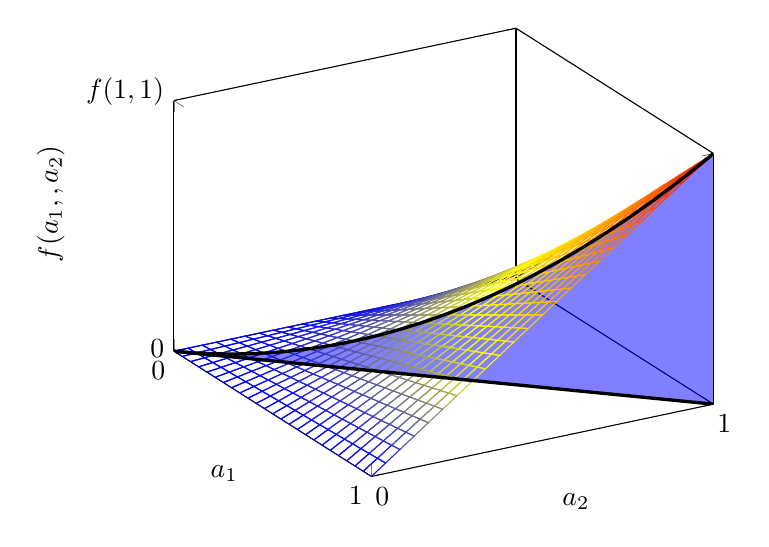
\begin{tikzpicture}
        \begin{axis}[
            xlabel={$a_1$}, ylabel={$a_2$}, zlabel={$f(a_1,, a_2)$},
            domain=0:1, y domain=0:1,
            zmin=0, zmax=1,
            xtick={0, 1}, ytick={0, 1}, ztick={0, 1},
            zticklabels={0, {$f(1, 1)$}}, % use the literal expression as a label
            view={60}{30}
        ]
            % plot the function
            \addplot3[surf, shader=flat, draw=none, name path=f, fill opacity=0] {x*y};
            % highlight the diagonal
            \addplot3[black, name path=diagonal, very thick, domain=0:1, samples=100, samples y=0] ({x}, {x}, {0});
            \addplot3[black, name path=f_diagonal, very thick, domain=0:1, samples=100, samples y=0] ({x}, {x}, {x^2});
            \addplot[blue, fill opacity=0.5] fill between[of=diagonal and f_diagonal];
        \end{axis}
    \end{tikzpicture}
    \caption{Illustration of the Shapley value in the case of two types of fringe players. The blue area corresponds to the value of the platform (with a scaling factor of $\sqrt{2}$ to account for the length of the diagonal)}
    \label{fig:many_sided_shapley}
\end{figure}


\subsection{Weighted value}

The final part of this section is dedicated to the weighted value in the many-sided case.
The set of players and the characteristic function are the same as in the previous section, but, as before, each player has a weight attached to them.
I will assume that fringe players are identical to each other within their types also with respect to their weights.
That is, the weight system for the game is the following: player $P$ has weight $\lambda_P$, while players $A^l_i$ have weight $\lambda_l$.

I will show, that as with non-weighted Shapley value, the limit of the weighted value can be expressed as an integral over a one-dimensional path in the weighted case as well.
However, now this path is not the diagonal of the unit hypercube, but a function of the fringe players' weights.
The reason for this is that not all permutations have the same probability of occurring: those with players having higher weights ordered later are more likely to occur.

The following statement is the central theorem of this paper.
In fact, most of the propositions in the previous sections can be considered as special cases of it.
\begin{theorem}
    \label{prop:many_sided_weighted}
    Let $f$ be continuous on $[0, 1]^L$.
    Then,
    \begin{align*}
        \varphi_P^\infty & = \int_0^1 \lambda_P t^{\lambda_P - 1} f(t^{\lambda_1}, \dots, t^{\lambda^L}) \dt
    \end{align*}
    and
    \begin{align*}
        \varphi_{A^l}^\infty & = \int_0^1 t^{\lambda_P} \lambda_l t^{\lambda_l - 1} \partial_l f(t^{\lambda_1}, \dots, t^{\lambda^L}) \dt.
    \end{align*}
\end{theorem}
The intuition is the following.
A higher weight for a player means that it has a higher chance of being relatively late in a random permutation.
Therefore, conditional on $s$ proportion of the fringe coming before $P$, the various types' proportions do not reflect their population shares ($1/L$).
For any $s \in (0, 1)$, the proportion of fringe players with a higher weight is lower than their population share, while the proportion of fringe players with a lower weight is higher than their population share.

Cref{fig:many_sided_weighted} illustrates this phenomenon in the case of two types of fringe players.
Fringe players of type $A^2$ have a higher weight than those of type $A^1$, and thus the path the integral is taken over contains more of the latter than the former.

Finally, player $P$'s probability of coming after $s$ proportion of the fringe is also not uniform, but rather influenced by the relationship between its own and the fringe players' weights.\footnote{
    This is the same mechanism as in the case of the one-sided weighted value.
}
Therefore, the integral is not taken with respect to the uniform distribution, but rather one resembling that of \cref{prop:one_sided_weighted}.
The result is the following: when the big player has a higher weight, its chances of being relatively late in the ordering are higher, and thus -- due to $f$ being monotone increasing -- its value is higher.
The following, simple corollary formalizes this idea.

\begin{figure}
    \centering
    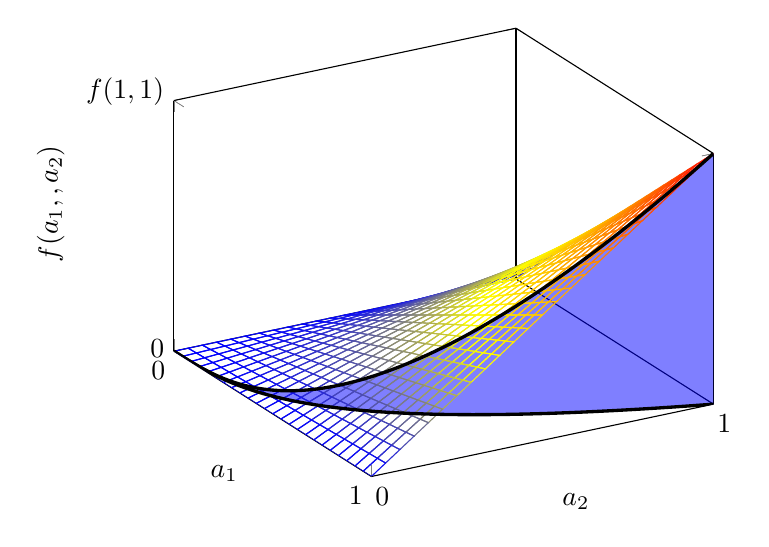
\begin{tikzpicture}
        \begin{axis}[
            xlabel={$a_1$}, ylabel={$a_2$}, zlabel={$f(a_1,, a_2)$},
            domain=0:1, y domain=0:1,
            zmin=0, zmax=1,
            xtick={0, 1}, ytick={0, 1}, ztick={0, 1},
            zticklabels={0, {$f(1, 1)$}}, % use the literal expression as a label
            view={60}{30}
        ]
            % plot the function
            \addplot3[surf, shader=flat, draw=none, name path=f, fill opacity=0] {x*y};
            % highlight the diagonal
            \addplot3[black, name path=diagonal, very thick, domain=0:1, samples=100, samples y=0] ({x}, {x^3}, {0});
            \addplot3[black, name path=f_diagonal, very thick, domain=0:1, samples=100, samples y=0] ({x}, {x^3}, {x^4});
            \addplot[blue, fill opacity=0.5] fill between[of=diagonal and f_diagonal];
        \end{axis}
    \end{tikzpicture}
    \caption{Illustration of the weighted value in the case of two types of fringe players. Players of type $A^2$ have a higher weight than those of type $A^1$, thus the integral is not taken over the diagonal. The blue area corresponds to the value of the platform (the area have to be scaled so that the length of the path integrated over is one)}
    \label{fig:many_sided_weighted}
\end{figure}

\begin{corollary}
    \label{cor:platform_value_multiple_sides_weighted}
    $\varphi_P^\infty$ is increasing in $\lambda_P$ unless $f$ is constant.
\end{corollary}
This result is analogous to \cref{cor:platform_value_weighted}, and demonstrates that a higher weight for player $P$ corresponds to a higher value in this game as well.

\section{Example application}

In this section I will apply the results of the previous sections to a simple model of two-sided platforms.
I follow the modelling approach of the monopoly platform case in \textcite{armstrong2006competition}, with a few extensions.
There are two major departures from the original model.
First, and most importantly, instead of letting the platform choose entry fees, I assume that they are the result of a bargaining process, and the outcomes are described by the weighted value.
Second, instead of assuming that each player's utility is linear in the number of the other side's players, I allow for more general (power) functions, which lets me capture the substitutability of the two sides.

\subsection{Model}

Imagine a two-sided market with a continuum of players on both sides.
Furthermore, assume that there is a single platform that connects the two sides.
The utility that a player on side $i$ derives from participating in the market is an increasing function\footnote{
    \textcite{armstrong2006competition} -- along with much of the literature on two-sided markets \parencite[e.g.][]{rochet2003platform,hagiu2006pricing} -- assumes that the utility of a player is linear in the number of players on the other side.
    Using a more general function allows me to model different degrees of network effects.
} of the number of players on the other side ($n_j$), minus the entry fee charged by the platform ($p_i$):
\begin{align*}
    u_i = \alpha_i n_j ^ {\gamma_i} - p_i,
\end{align*}
where $\alpha \geq 0$ and $\gamma > 0$ determine the strength and shape of the network effects, respectively.

Following \textcite{armstrong2006competition}, let us also model player entry in a reduced form manner.
Assume that there is a continuum of potential entrants on both sides of the market.
The number of actual entrants depends on the utility they would derive from participating in the market.\footnote{
    Such assumptions are usually justified by some idiosyncratic cost of entry, the distribution of which determines the function $\phi$.
    In the main text, for simplicity, I refrain from explicitly modeling this cost, but \cref{sec:explicit_entry_costs} provides a discussion of how to incorporate it into the model, and how it would affect bargaining outcomes.
}
Let us denote this relationship as $\phi_i(u_i)$, where $\phi_i$ is a strictly increasing, differentiable function.
Then,
\begin{align*}
    n_i = \phi_i(u_i).
\end{align*}

Finally, let us assume that the platform can charge lump-sum entry fees to both sides.
These fees can also be negative, in which case they are interpreted as subsidies.
The platform's profit is the sum of entry fees, minus the cost of serving the entrants ($F_i$ for each entrant):
\begin{align*}
    \pi(n_1, n_2) = n_1 p_1 + n_2 p_2 - F_1 n_1 - F_2 n_2.
\end{align*}

I will consider two cases as to the timing and nature of the price-setting process, as well as a welfare-maximizing benchmark.
For the latter, I derive the entry fees that maximize social welfare, i.e. the sum of the utilities of the two sides plus the platform's profit.
After that, I will first consider a model analogous to that in \textcite{armstrong2006competition}, where the platform can unilaterally commit to any entry fees it wishes.
Finally, I consider a model in which entry fees are the result of a bargaining process in such a way that the resulting utilities and profits correspond to the various players' weighted values.

\subsection{Benchmark: welfare-maximizing entry fees}

Let us consider first what entry fees would maximize social welfare.
Instead of approaching this problem directly, let us rely on the following observation: if entry fees correspond to the externality that a player's entry imposes on the other side, then the resulting choices are welfare-maximizing.
In this specific case, there are two externalities to consider.
First, it costs the platform $F_i$ to serve an additional player on side $i$.
Second, the entry of a player on side $i$ increases the utility on side $j$ due to positive network effects.
Welfare is maximized when the price reflects the balance of these two  factors:
\begin{align*}
    p_i^* &= F_i - n_j \frac{\partial u_j}{\partial n_i} \\
          &= F_i - \alpha_j \gamma_j n_j n_i^{\gamma_j - 1}.
\end{align*}
As in \textcite{armstrong2006competition}, for any $\alpha_j > 0$ welfare-maximizing $F_i$ is below the platform's cost of serving player $i$.
Thus, the platform's profit would necessarily be negative.
It naturally cannot happen in the case when the platform sets the entry fees, or even the bargaining case.

As an immediate corollary, utilities in this case are given by
\begin{align*}
    u_i^*(n_i, n_j) = \alpha_i n_j ^ {\gamma_i} + \alpha_j \gamma_j n_j n_i^{\gamma_j - 1} - F_i
\end{align*}
for an individual player on side $i$.
That is, side $i$ obtains the total utility generated by its players minus the cost of serving them, plus $\gamma_j$ times the total utility generated by the other side, too. This is due to the positive externality that side $i$ imposes on side $j$.

Furthermore, the utility of type $i$ depends positively on both $\alpha_i$ (mechanically) and $\alpha_j$ (a stronger positive externality on the other players implies a lower entry fee and thus higher utility).
Finally, if $n_i \geq e^{-\frac{1}{\gamma_j}}$, then $u_i$ is also increasing in $\gamma_j$.
Both of the latter two effects are related to player $i$ being compensated for the positive externality it imposes on the other side.

One can also obtain the total welfare of side $i$, as it is simply the number of entrants times the non-idiosyncratic utility of its players, plus the sum (integral) of the idiosyncratic utilities.
\begin{align}
    \label{eq:W_star}
    W_i^*(n_i, n_j) = \alpha_i n_i n_j ^ {\gamma_i} + \gamma_j \alpha_j n_j n_i^{\gamma_j} - n_i F_i.
\end{align}

\subsection{Platform sets prices unilaterally}

Now let us examine what happens when the platform sets the entry fees unilaterally.
First, rewrite the platform's profit as a function of utilities, rather than the number of entrants:
\begin{align*}
    \pi(u_1, u_2) = \phi_1(u_1) [\alpha_1 \phi_2(u_2) ^ {\gamma_1} - u_1 - F_1] + \phi_2(u_2) [\alpha_2 \phi_1(u_1) ^ {\gamma_2} - u_2 - F_2].
\end{align*}

Let us assume that the above expression is concave, and thus the first order conditions characterize its maximum.
Then, simply taking the partial derivatives with respect to $u_i$ yields the following condition for the optimal entry fees.
\begin{proposition}
    \label{prop:platform_unilateral}
    If the platform can set entry fees unilaterally, then optimal entry fees for side $i$ are characterized by
    \begin{align*}
        p_i^u &= F_i - \alpha_j \gamma_j n_j n_i^{\gamma_j - 1} + \frac{\phi_1(u_1)}{\phi'_1(u_1)} \\
              &= p_i^* + \frac{\phi_1(u_1)}{\phi'_1(u_1)}.
    \end{align*}
\end{proposition}

As one would expect, profit-maximizing entry fees are higher than welfare-maximizing ones.
In addition to the comparative statics of the welfare-maximizing case, the platform's entry fees also depend on the elasticity of entry.
When it is low, the platform will set a high entry fee, as the loss of entrants is small.

For ease of comparison with the bargaining case, let us also derive the utilities in this case:
\begin{align*}
    u_i^u(n_1, n_2) &= \alpha_i n_j ^ {\gamma_i} + \alpha_j \gamma_j n_j n_i^{\gamma_j - 1} - F_i - \frac{\phi_1(u_i)}{\phi'_1(u_i)}
\end{align*}
Welfare of side $i$ immediately follows in this case, too:
\begin{align*}
    \label{eq:W_u}
    W_i^u(n_1, n_2) = \alpha_i n_i n_j ^ {\gamma_i} + \gamma_j \alpha_j n_j n_i^{\gamma_j} - n_i F_i - n_i^2 (\phi_i^{-1})'(n_i).
\end{align*}
Clearly, equilibrium utilities must be smaller than in the welfare-maximizing case.
Due to $\phi_i$ being increasing, the number of entrants is also lower.

\subsection{Bargaining}

Finally, let us consider the case when the platform and the players bargain over the value they generate.
Assume that $n_1$ and $n_2$ players have decided to enter on sides $1$ and $2$, respectively.
Furthermore, assume that players' bargaining weights are $\lambda_1, \lambda_2$ and $\lambda_P$.

The characteristic function of the game takes a similar form to that in \cref{sec:many_sided}.
If the platform is not part of the coalition, then the value the coalition can generate is zero.
Otherwise, it is simply the sum of the utilities of the two sides minus the cost of serving them.\footnote{
    Entry fees do not matter, as they are within-coalition transfers, and thus do not affect the total value.
}
This value, as a function of the number of entrants, is
\begin{align*}
    w(n_1, n_2) = n_1 \alpha_1 n_2^{\gamma_1} + n_2 \alpha_2 n_1^{\gamma_2} - F_1 n_1 - F_2 n_2.
\end{align*}

The share received by each type of player is then easily established using \cref{prop:many_sided_weighted}.
\begin{proposition}
    \label{prop:platform_bargaining_last_period}
    The weighted values of the various sides without idiosyncratic costs are
    \begin{alignat*}{4}
        \pi_P^b(n_1, n_2) &= \underbracket{\frac{\lambda_P}{\lambda_P + \lambda_1 + \lambda_2\gamma_1}}_{\coloneqq S_P^{b_1}} \alpha_1 n_1 n_2^{\gamma_1} &&+ \underbracket{\frac{\lambda_P}{\lambda_P + \lambda_2 + \lambda_1\gamma_2}}_{\coloneqq S_P^{b_2}} \alpha_2 n_2 n_1^{\gamma_2} &&- \underbracket{\frac{\lambda_P}{\lambda_P + \lambda_1}}_{\coloneqq S_P^{c_1}} n_1 F_1 &&- \underbracket{\frac{\lambda_P}{\lambda_P + \lambda_2}}_{\coloneqq S_P^{c_2}} n_2 F_2 \\
        w_1^b(n_1, n_2) &= \underbracket{\frac{\lambda_1}{\lambda_P + \lambda_1 + \lambda_2\gamma_1}}_{\coloneqq S_1^{b_1}} \alpha_1 n_1 n_2^{\gamma_1} &&+ \underbracket{\frac{\lambda_1 \gamma_2}{\lambda_P + \lambda_2 + \lambda_1\gamma_2}}_{\coloneqq S_1^{b_2}}  \alpha_2 n_2 n_1^{\gamma_2} &&- \underbracket{\frac{\lambda_1}{\lambda_P + \lambda_1}}_{\coloneqq S_1^{c_1}} n_1 F_1 && \\
        w_2^b(n_1, n_2) &= \underbracket{\frac{\lambda_2\gamma_1}{\lambda_P + \lambda_1 + \lambda_2\gamma_1}}_{\coloneqq S_2^{b_1}} \alpha_1 n_1 n_2^{\gamma_1} &&+ \underbracket{\frac{\lambda_2}{\lambda_P + \lambda_2 + \lambda_1\gamma_2}}_{\coloneqq S_2^{b_1}} \alpha_2 n_2 n_1^{\gamma_2} && &&- \underbracket{\frac{\lambda_2}{\lambda_P + \lambda_2}}_{\coloneqq S_2^{c_2}} n_2 F_2.
    \end{alignat*}
\end{proposition}

There are four parts that the total welfare $w(n_1, n_2)$ is divided into: utility generated by side $1$ and $2$, and cost of serving side $1$ and $2$.
Each side's share of these parts is given by $S_i^{b_1}, S_i^{b_2}, S_i^{c_1}$ and $S_i^{c_2}$, respectively.
As it turns out, these shares only depend on the bargaining weights ($\lambda_P, \lambda_1, \lambda_2$) and the network effects ($\gamma_1, \gamma_2$), but not on the actual number of entrants.\footnote{
    This is due to the characteristic function being a polynomial in the number of entrants.
    Just like in \cref{sec:power_function_example}, the parts of the polynomial are divided in a constant proportion.
}
Furthermore, all of these shares are increasing in one's own bargaining weight, and decreasing in the others' weights.
Finally, the share of side $i$ from the value generated on side $j$ is also increasing in $\gamma_j$.
This means that if players on side $i$ are less substitutable / more complementary in terms of generating utility on side $j$, then they will receive a larger share of the value generated on that side.

These utilities are remarkably similar in structure to the welfare maximizing case in \cref{eq:W_star}.
The main difference is that each part (both costs and positive utilities) is reweighted, and side $i$ only receives a fraction of it.
It is also worth noting that $W_i^b(n_1, n_2) < W_i^*(n_1, n_2)$, and, as a consequence, entry is lower than what would be socially optimal.\footnote{
    The easiest way to see it is that in the welfare-maximizing case the platform's profit is negative, while in the bargaining case it is positive.
    Therefore, fringe utilities must be lower in the latter case.
}

For better comparison, let us also examine implied entry fees and non-idiosyncratic utilities.
The latter is the difference between the average welfare and the average idiosyncratic cost:
\begin{align*}
    u_i^b(n_1, n_2) &= \frac{\lambda_i}{\lambda_P + \lambda_i + \lambda_j\gamma_i} \alpha_i n_j^{\gamma_i} + \frac{\lambda_i \gamma_j}{\lambda_P + \lambda_j + \lambda_i\gamma_j} \alpha_j n_j n_i^{\gamma_j - 1} - \frac{\lambda_i}{\lambda_P + \lambda_i} F_i.
\end{align*}
If one wished to close the model, the number of entrants in equilibrium could be obtained by solving the system of equations $n_i = \phi_i(u_i(n_1, n_2)), n \in \{1, 2\}$.
Finally, the implied entry fees can be calculated from the equation $u_i = \alpha_i n_j^{\gamma_i} - p_i$, yielding
\begin{align*}
    p_i^b(n_1, n_2) &= \frac{\lambda_i}{\lambda_P + \lambda_i} F_i - \frac{\lambda_i \gamma_j}{\lambda_P + \lambda_j + \lambda_i\gamma_j} \alpha_j n_j n_i^{\gamma_j - 1} + \frac{\lambda_P + \lambda_j\gamma_i}{\lambda_P + \lambda_i + \lambda_j\gamma_i} \alpha_i n_j^{\gamma_i}.
\end{align*}

\subsection{Comparison}

Let us now compare the outcomes of the three cases described in this section.
To highlight the similarity to \textcite{armstrong2006competition}, I will first consider the case of linear network effects.
Furthermore, for simplicity of exposition, I start by considering the non-weighted Shapley value before moving on to the weighted value.

Assume that network effects are linear, i.e. $\gamma_i = 1$ for $i \in \{1, 2\}$.
Also, focus on non-weighted Shapley values ($\lambda_P = \lambda_1 = \lambda_2 = 1$).
From the previous results, the entry fees for side $i$ are
\begin{align*}
    p_i^* &= \underbracket{F_i}_{(1)} - \underbracket{\alpha_j n_j n_i}_{(2)}, \\
    p_i^u &= \underbracket{F_i}_{(1)} - \underbracket{\alpha_j n_j n_i}_{(2)} + \underbracket{n_i (\phi_i^{-1})'(n_i)}_{(3)} \\
    p_i^b &= \underbracket{\frac{1}{2} F_i}_{(1)} - \underbracket{\frac{1}{3} \alpha_j n_j n_i}_{(2)} + \underbracket{\frac{2}{3} \alpha_i n_j}_{(4)},
\end{align*}
for the welfare-maximizing, unilateral price setting and bargaining cases, respectively.

All of these expressions bear some similarities to each other, in that the price is somehow related to the externalities that an entrant imposes on the other players.
In fact, the welfare-maximizing price is just that: the cost of serving one additional player (1) and the positive externality imposed on the other side (2).
The unilateral pricing case also includes these two factors in full, but also adds a third factor, related to the elasticity of entry (3).
Namely, the platform extracts some of the surplus generated by the entrants, and the surplus it can extract depends on $\phi'_i(u_i)$.
It is the same mechanism that leads to markups in a simple monopolistic pricing model.

The bargaining case also includes the first two factors, albeit they are somewhat different.
As opposed to the first two cases, the price only contains some fraction of the externalities, and the rest is shared with the platform and the other side.\footnote{
    Due to the linearity of the model, various parts of the value are shared equally between players who participate in producing them.
    This is the reason why, for example, the platform and the firms share the cost of serving the entrants (1) equally, or that all three types of players share the value generated on a given side (2) equally.
}
Furthermore, some part of the welfare generated on side $i$ is also shared with the other players, and thus appears in the price (4).
This is in contrast to both the welfare-maximizing and unilateral pricing cases, where the entry fee did not depend on the actual utility that was materialized on the given side.
Therefore, bargaining introduces some interesting departures from both the welfare-maximizing and unilateral pricing cases.

Now let us consider non-linear network effects.
The welfare-maximizing, unilateral pricing and bargaining entry fees are as follows:
\begin{align*}
    p_i^* &= \underbracket{F_i}_{(1)} - \underbracket{\alpha_j \gamma_j n_j n_i^{\gamma_j - 1}}_{(2)}, \\
    p_i^u &= \underbracket{F_i}_{(1)} - \underbracket{\alpha_j \gamma_j n_j n_i^{\gamma_j - 1}}_{(2)} + \underbracket{n_i \kappa'_i(n_i)}_{(3)} \\
    p_i^b &= \underbracket{\frac{1}{2} F_i}_{(1)} - \underbracket{\frac{\gamma_j}{2 + \gamma_j} \alpha_j n_j n_i^{\gamma_j - 1}}_{(2)} + \underbracket{\frac{1 + \gamma_i}{2 + \gamma_i} \alpha_i n_j^{\gamma_i}}_{(4)}.
\end{align*}
For the most part, the intuition is the same as in the linear case.
The welfare-maximizing price is still the cost of serving one additional player (1) and the positive externality imposed on the other side (2).
In addition to those, the unilaterally set entry fee includes a markup related to the elasticity of entry (3).
Finally, in the case of bargaining, these factors do not appear in full, but are shared with the platform and the other side.

There is one important difference in the bargaining case, however.
In the linear case, the terms related to the value generated on each side were shared between the players in a constant proportion, independent of the model parameters.
In the non-linear case, however, these shares do depend on the shape of the network effects.
In particular, when side $i$'s network externality on side $j$ is more convex (e.g. firms on side $i$ are less substitutable), then it receives a larger share of the value generated on the other side.
This is signified by the fact that the coefficient of side $i$'s network externality, $\frac{\gamma_j}{2 + \gamma_j}$, is increasing in $\gamma_j$.
This result shows that the bargaining outcomes are not just a trivial distribution of the value, but also take into account the shape of the network effects.

Finally, for completeness, let us consider the case of weighted values.
The following theorem summarizes the entry fees in this most general case.
\begin{theorem}
    Let $p_i^*$, $p_i^u$ and $p_i^b$ denote the welfare-maximizing, unilateral pricing and bargaining entry fees, respectively.
    Then,
    \begin{align*}
        p_i^* &= \underbracket{F_i}_{(1)} - \underbracket{\alpha_j \gamma_j n_j n_i^{\gamma_j - 1}}_{(2)}, \\
        p_i^u &= \underbracket{F_i}_{(1)} - \underbracket{\alpha_j \gamma_j n_j n_i^{\gamma_j - 1}}_{(2)} + \underbracket{n_i \kappa'_i(n_i)}_{(3)} \\
        p_i^b &= \underbracket{\frac{\lambda_i}{\lambda_P + \lambda_i} F_i}_{(1)} - \underbracket{\frac{\lambda_i \gamma_j}{\lambda_P + \lambda_j + \lambda_i\gamma_j} \alpha_j n_j n_i^{\gamma_j - 1}}_{(2)} + \underbracket{\frac{\lambda_P + \lambda_j\gamma_i}{\lambda_P + \lambda_i + \lambda_j\gamma_i} \alpha_i n_j^{\gamma_i}}_{(4)}.
    \end{align*}
\end{theorem}

In the case of the linear terms, such as the cost of serving one additional player (1), the addition of bargaining weights simply leads to players shareing the cost in a constant proportion, according to their weights.
The higher the weight, the larger the share for the player.
While the latter is true for non-linear terms, as well, the influence of the weights is more complex, as it also depends on the shape of value function.
For example, in term (2), $\lambda_i$ interacts with the parameter determining the shape of the network effects, $\gamma_j$
Therefore, the weighted value is more than just a simple reweighting of the non-weighted value, and its effects can be quite complex depending on the assumptions on the value function.

Whether bargaining leads to a higher or lower total welfare depends on the parameters of the model.
For example, if $\lambda_P$ is very high, then $p_i^b > p_i^u > p_i^*$, leading to fewer firms entering and lower total surplus than not only the welfare-maximizing case, but also the unilateral pricing case.
That is, everybody looses from bargaining.\footnote{
    In such a case, the platform would like to set lower entry fees that what it can achieve via bargaining.
    While in some settings it is very plausible that it can do it, in others commitment problems might prevent it from doing so.
}

On the other hand, if $\lambda_P$ is sufficiently low, then one can find weights $\lambda_1, \lambda_2$, such that $p_i^u > p_i^b > p_i^*$.
In such a case, the platform would like to set higher entry fees than what it can achieve via bargaining.
The total welfare is also between the welfare-maximizing and unilateral pricing cases, therefore bargaining can be beneficial as an alternative of unilateral pricing.
The platform, however, achieves a lower profit than if it could set the entry fees unilaterally.

Finally, it is always true that $p_1^b < p_1^*$ or $p_2^b < p_2^*$.
The reason is that the platform's profit is always non-negative in the bargaining case, while it is negative in the welfare-maximizing case.
This also implies that the total welfare is strictly lower than in the welfare-maximizing case.
Therefore, while bargaining can be welfare-increasing compared to unilateral price setting, it can not achieve the highest possible total welfare.\footnote{
    One could argue that the welfare maximizing case is not a realistic benchmark anyway, as it assumes that the platform is making a loss.
}

\section{Conclusions}

In this paper, I examined the problem of bargaining between one indispensable player and a continuum of fringe players.
I did so using the concept of random order values from cooperative game theory.
I showed that random-order-value-based bargaining has some desirable properties, and that it coincides with intuitive expectations in terms of certain comparative statics.
Furthermore, the resulting distributions of the value are also analytically tractable, and has neat geometric interpretations.

I use random order values to provide a comprehensive framework for a number of important special cases.
Some of those, such as the Shapley-value, or the weighted value in the one-sided case, is already known in the literature.\footnote{
    Aside from looking at it in an abstract manner, my contribution to those cases mostly lie in showing how the fringe's value can be expressed as a kind of expected marginal contribution.
    This is especially relevant in the multi-sided case, where it is important to know how the value not obtained by the indispensible player is distributed among the various sides.
}
Others, such as the weighted value in the multi-sided case, or the interpretation of substitutable "indispensible" players, are, to the best of my knowledge, new.
As I demonstrate, they retain the simplicity and interpretability of the simpler cases, while making the model more general.
Finally, I demonstrate how the proposed framework can be applied in practice by
examining the two-sided platform model of \textcite{armstrong2006competition} with a small extension and a bargaining process over entry fees.
I show that the resulting entry fees have a simple structure, but they also differ from the welfare-maximizing and unilateral price-setting cases in number of interesting ways.
Therefore, in situations where bargaining between players is plausible, certain effects might be missed if one assumes unilateral price-setting.

There is a variety of ways in which this paper could be expanded or built upon.
One obvious direction is to consider other solution concepts from cooperative game theory, such as the nuclelous\footnote{
    It retains many of the desirable properties of the Shapley-value, such as existence and uniqueness, but it is contained in the core when the latter exists, and thus has a more immediate connection to non-cooperative bargaining theory.
}.
Another way to go is to build non-cooperative microfoundations for the random-order-value-based bargaining outcomes.
Many such results exist for the Shapley value, and some also exist for the weighted value, but it might be interesting to see if some of the more general random order values can be motivated in a similar manner.

Besides those theoretical directions, the practical applications are no less interesting.
The proposed profit sharing framework could be embedded in more realistic models of various settings.
The example application in this paper is a streamlined example of this, while \textcite{stancsics2023hybrid} provides a more detailed model involving hybrid platforms.
Due to the simplicity of the results, this approach might be a viable replacement of unilateral price setting in cases where one does not wish to ascribe all the bargaining power to one player.


\appendix

\printbibliography


\section{Non-indispensable big player(s)}
\label{sec:extensions}

This section demonstrates two ways in which the model can be extended to include non-indispensable big players, while retaining the essential structure and the tractability of the results.
In the first case, there are a number of big players, which are perfect substitutes of each other.
In the second case, there is a single big player, the fringe is able to generate some value on its own, and the big player is only needed to generate the rest.
In both cases, the value function is still a random order value, and thus results from the main text can be applied.

\subsection{Shapley value with multiple big players}

Now imagine that, instead of just one, there are $m$ players of type $P$, and they are perfect substitutes of each other.
That is, the fringe players still need one at least of them to achieve any value, but it does not matter which and how many of them are present.
Formally, the value function for coalition $S$ becomes the following:
\begin{align*}
    v(S) = \begin{cases}
        0                              & \text{if } n_P(S) = 0 \\
        f\left(\frac{n_A(S)}{n}\right) & \text{otherwise}.
    \end{cases}
\end{align*}

Let us start by establishing monotonicity for this version of the model, too.
\begin{proposition}
    The game is monotone if $f$ is increasing and $f(0) \geq 0$.
\end{proposition}
On the other hand, superadditivity is not as simple in this case, as before.
For example, when $f$ is concave, then $m$ coalitions with one platform each and the fringe divided equally amongst them clearly achieve a higher total payoff than the grand coalition.
Therefore, the results of this section are most applicable to settings when multiple coalitions cannot be formed at the same time for some reason.
For example, \textcite{hart1996bargaining} propose an interpretation when there is a single, indivisible, non-replicable resource or technology (not captured in the value function) necessary to produce any value.

As before, the main proposition in this section provides us with an expression of the limit of the value for this variant of the game.
Notably, as in the case of the weighted value, the share of player $P$ can again be expressed as an integral of $f$ and some weighting\footnote{
    Weighting is not a completely precise term, as $h(t)$ does not integrate to one, and is therefore not a probability distribution in this case (\cref{fig:multiple_platforms}).
} function $h(t)$, with the latter depending only on the number of big players.
\begin{proposition}
    \label{prop:multiple_platforms}
    The limit of the Shapley-value (as $n \to \infty$) of each player of type $P$ is
    \begin{align*}
        \varphi_{P_i}^{\infty, m} = \int_0^1 h(t) f(t) \dt,
    \end{align*}
    where $h(t) = (1-t) ^ {m-1}$.
\end{proposition}

As with proposition \ref{prop:one_sided}, this result also has a probabilistic interpretation.
Let the location of the $m$ atoms be $t_1, \dots, t_m$, distributed independently and uniformly on the unit interval.
The expected marginal contribution of $t_i$ is only positive whenever it is the first amongst the major players.
That is, for any $t_i$, the probability if $P_i$ being the first is related to the cdf of the first order statistic from $n-1$ independent uniform distributions: $1 - (1-t)^{m-1}$.

\begin{figure}[ht]
    \centering
    \begin{subfigure}[b]{0.45\textwidth}
        \centering
        \begin{tikzpicture}[scale=0.8]
            \begin{axis}[xmin=0, xmax=1, ymin=0, ymax=1.1, samples at={0, 0.02, 0.04, ..., 0.98, 1},
                xtick={0, 1}, ytick={0, 1}, axis lines=left, xlabel={$t$}, legend pos=north west]
                \addplot[thick] {1};
                \addplot[thick, dashed] {1-x};
                \addplot[thick, dotted] {(1-x)^2};
            \end{axis}
        \end{tikzpicture}
        \caption{$h(t)$}
    \end{subfigure}
    \begin{subfigure}[b]{0.45\textwidth}
        \centering
        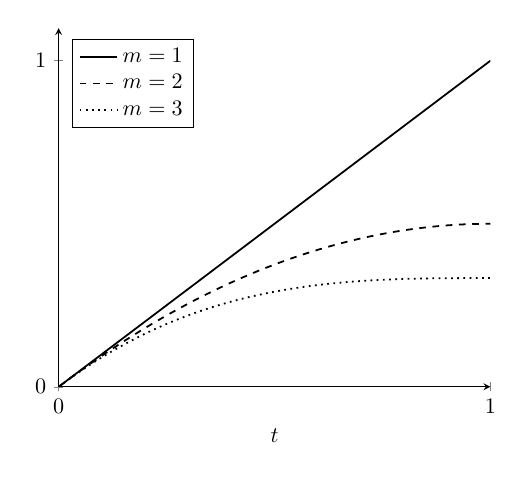
\begin{tikzpicture}[scale=0.8]
            \begin{axis}[xmin=0, xmax=1, ymin=0, ymax=1.1, samples at={0, 0.02, ..., 0.98, 1},
                xtick={0, 1}, ytick={0, 1}, axis lines=left, xlabel={$t$}, legend pos=north west]
                \addplot[thick] {x};
                \addplot[thick, dashed] {x - x^2/2};
                \addplot[thick, dotted] {x - x^2 + x^3/3};
                \legend{$m = 1$, $m = 2$, $m = 3$}
            \end{axis}
        \end{tikzpicture}
        \caption{$\int_0^t h(s) \ds$}
    \end{subfigure}
    \caption{Illustration of the weighting function for various values of $m$ in the multiple big player case -- individual big player.}
    \label{fig:multiple_platforms}
\end{figure}

Let us examine the total value of all the big players.
Denote the aggregated value of players of type $P$ as $\varphi_{P}^{\infty, m} \coloneqq \sum_{j=1}^m\varphi_{P_j}^{\infty, m} = m\varphi_{P_i}^{\infty, m}$.
It immediately follows from the previous proposition that
\begin{align*}
    \varphi_{P}^{\infty, m} = \int_0^1 g(t) f(t) \dt,
\end{align*}
where $g(t) = m (1-t) ^ {m-1}$.
Notice that $g(t)$ now integrates to one, and is thus a probability distribution (\cref{fig:multiple_platforms_total}).
Therefore, the Shapley value in the case of multiple, substitutable big players can be interpreted as a random order value with a single big player.
The probability distribution for the corresponding random order value has a specific form, and its only parameter is the number of big players.
Thus, all the results from the previous section apply to this case as well.

\begin{figure}[ht]
    \centering
    \begin{subfigure}[b]{0.45\textwidth}
        \centering
        \begin{tikzpicture}[scale=0.8]
            \begin{axis}[xmin=0, xmax=1, ymin=0, ymax=3.1, samples at={0, 0.02, 0.04, ..., 0.98, 1},
                xtick={0, 1}, ytick={0, 1, 2, 3}, axis lines=left, xlabel={$t$}, legend pos=north west]
                \addplot[thick] {1};
                \addplot[thick, dashed] {2 * (1-x)};
                \addplot[thick, dotted] {3 * ((1-x)^2)};
            \end{axis}
        \end{tikzpicture}
        \caption{$g(t)$}
    \end{subfigure}
    \begin{subfigure}[b]{0.45\textwidth}
        \centering
        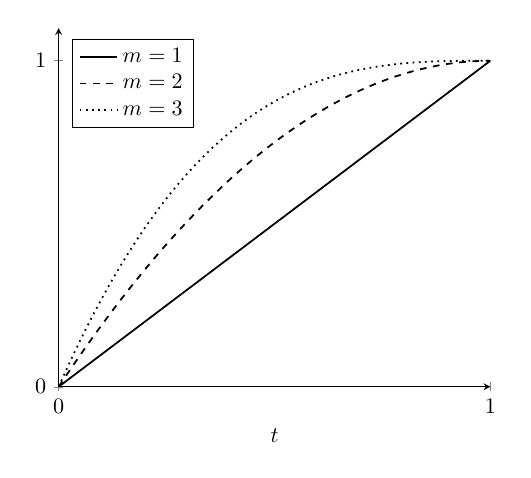
\begin{tikzpicture}[scale=0.8]
            \begin{axis}[xmin=0, xmax=1, ymin=0, ymax=1.1, samples at={0, 0.02, ..., 0.98, 1},
                xtick={0, 1}, ytick={0, 1}, axis lines=left, xlabel={$t$}, legend pos=north west]
                \addplot[thick] {x};
                \addplot[thick, dashed] {2 * (x - x^2/2)};
                \addplot[thick, dotted] {3 * (x - x^2 + x^3/3)};
                \legend{$m = 1$, $m = 2$, $m = 3$}
            \end{axis}
        \end{tikzpicture}
        \caption{$\int_0^t g(s) \ds$}
    \end{subfigure}
    \caption{Illustration of the weighting function for various values of $m$ in the multiple big player case -- total of big players.}
    \label{fig:multiple_platforms_total}
\end{figure}

Now let us look at how the value of the big players and the fringe changes as a function of the number of the big players.
Proposition \cref{cor:multiple_platforms_2} again confirms our intuition: more players means that they become more substitutable, and thus their bargaining power decreases.
This not only means that the value of each individual big player decreases, but also that their total value goes down.

\begin{corollary}
    \label{cor:multiple_platforms_2}
    Let $\varphi_{P}^{\infty, m} = m\varphi_{P_i}^{\infty, m}$ denote the aggregated values of players of type $P$. $\varphi_{P}^{\infty, m}$ is decreasing in $m$ and $\varphi_{A}^{\infty, m}$ is increasing in $m$ unless $f$ is constant.
\end{corollary}

Finally, let us show that the value of the fringe has a similar, marginal contribution-based interpretation as in the case of a single big player.

\begin{corollary}
    \label{cor:multiple_platforms}
    The per-unit Shapley-value of the fringe is
    \begin{align*}
        \varphi_A^{\infty, m} = 1 - \int_0^1 f(t) \dG(t) = \int_0^1 G(t) f'(t) \dt ,
    \end{align*}
    where $G(t) = 1 - (1-t)^m$.
\end{corollary}


\subsection{Small players can generate some value on their own}

As a final extension for the one-sided case, let us examine what happens when the small players can generate some value on their own.
Assume that the big player still provides some value to any coalition, but a coalition of fringe players can achieve a positive value even without it.
Formally, the value function is the following:
\begin{align*}
    v(S) = \begin{cases}
        f_0\left(\frac{n_A(S)}{n}\right) & P \notin S \\
        f\left(\frac{n_A(S)}{n}\right)   & \text{otherwise}.
    \end{cases}
\end{align*}

As in the case of multiple big players, monotonicity is straightforward to establish.
\begin{proposition}
    The game is monotone if $f$ is increasing and $f(t) \geq f_0(t) \geq 0 \forall t$.
\end{proposition}
Also similarly, superadditivity is not straightforward in general.
Therefore, the simultaneous formation of multiple coalitions must be excluded in this setting as well.

On the other hand, the random order values and their limits are very straightforward to characterize.
The value of the big player is still its average marginal contribution.
The only difference is that this marginal contribution (conditional on $s$ share of the fringe coming before $P$) is not simply $f(s)$, but rather $f(s) - f_0(s)$.
This is because the big player is not indispensable, and thus the fringe can achieve some value without it.

\begin{proposition}
    \label{prop:one_sided_non_indispensable}
    Let $f$ be continuous on [0, 1]. Furthermore, let us denote the random variable $\frac{|\mathcal{P}_P|}{n}$ as $X_n$. Assume that $X_n \xrightarrow[]{d} X$ with cdf $G_X(t)$ and (if exists) pdf $g(t)$.
    Then
    \begin{align*}
        \varphi_P^\infty = \lim_{n \to \infty} \varphi_P^n = \int_0^1 f(t) \dG(t) = \int_0^1 g(t) [f(t) - f_0(t)] \dt,
    \end{align*}
    with the last equality holding if $X$ is a continuous random variable.
\end{proposition}

The value of the fringe is also similar to the baseline case, except now fringe players have a non-zero marginal contribution even when $P$ is not present.
Therefore, there is an additional term in the integral, corresponding to the marginal value of the fringe when $P$ is not present.

\begin{corollary}
    \label{cor:fringe_value_non_indispensable}
    The aggregated value of the fringe is
    \begin{align*}
        \varphi_A^\infty = f(1) - \int_0^1 f(t) - f_0(t) \dG(t).
    \end{align*}
    Furthermore, if $f$ and $f_0$ are differentiable on $[0, 1]$, then the value of the fringe can also be expressed as
    \begin{align*}
        \varphi_A^\infty = \int_0^1 G(t) f'(t) + (1 - G(t)) f'_0(t) \dt.
    \end{align*}
\end{corollary}

It is clear that the value of the big player is decreasing in $f_0$ (\cref{fig:non_indispensable}).
Consequently, the value of the fringe is increasing in $f_0$, which is essentially its outside option (what it can achieve without the big player).
This is a natural result, and again, it is in line with what one would expect from bargaining theory.
\begin{figure}
    \centering
    \begin{subfigure}[b]{0.45\textwidth}
        \centering
        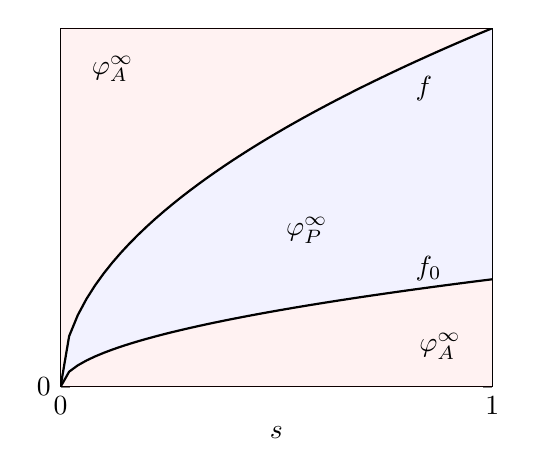
\begin{tikzpicture}[scale=0.8]
            \begin{axis}[xmin=0, xmax=1, ymin=0, ymax=1, samples at={0, 0.02, ..., 0.98, 1},
                    xtick={0, 1}, ytick={0}, xlabel={$s$}]
                \addplot[name path=f, thick] {x^0.5};
                \addplot[name path=f0, thick] {0.3 * x^0.5};
                \node[anchor=north west] at (axis cs: .8, .8^0.5) {$f$};
                \node[anchor=south west] at (axis cs: .8, .3*.8^0.5) {$f_0$};
                \path[name path=bottom] (axis cs:0,0) -- (axis cs:1,0);
                \path[name path=top] (axis cs:0,1) -- (axis cs:1,1);

                \addplot [fill=blue, fill opacity=0.05] fill between [of=f and f0];
                \addplot [fill=red, fill opacity=0.05] fill between [of=f and top];
                \addplot [fill=red, fill opacity=0.05] fill between [of=f0 and bottom];

                \node[anchor=north west, align=left] at (axis cs: .05, .95) {$\varphi_A^\infty$};
                \node[anchor=south east, align=left] at (axis cs: .95, .05) {$\varphi_A^\infty$};
                \node[anchor=north west, align=right] at (axis cs: .5, .5) {$\varphi_P^\infty$};
            \end{axis}
        \end{tikzpicture}
        \caption{Fringe can achieve relatively little without $P$}
    \end{subfigure}
    \begin{subfigure}[b]{0.45\textwidth}
        \centering
        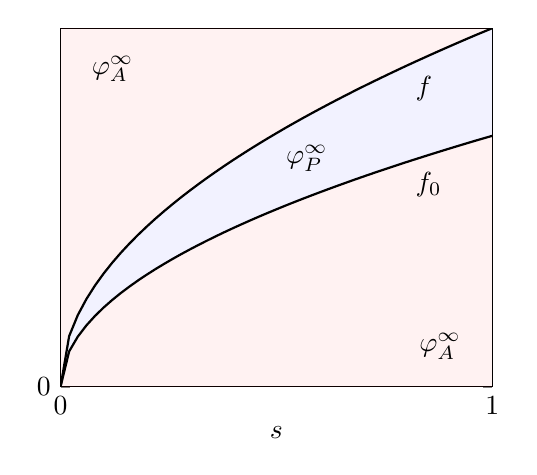
\begin{tikzpicture}[scale=0.8]
            \begin{axis}[xmin=0, xmax=1, ymin=0, ymax=1, samples at={0, 0.02, ..., 0.98, 1},
                    xtick={0, 1}, ytick={0}, xlabel={$s$}]
                \addplot[name path=f, thick] {x^0.5};
                \addplot[name path=f0, thick] {0.7 * x^0.5};
                \node[anchor=north west] at (axis cs: .8, .8^0.5) {$f$};
                \node[anchor=north west] at (axis cs: .8, .7*.8^0.5) {$f_0$};
                \path[name path=bottom] (axis cs:0,0) -- (axis cs:1,0);
                \path[name path=top] (axis cs:0,1) -- (axis cs:1,1);

                \addplot [fill=blue, fill opacity=0.05] fill between [of=f and f0];
                \addplot [fill=red, fill opacity=0.05] fill between [of=f and top];
                \addplot [fill=red, fill opacity=0.05] fill between [of=f0 and bottom];

                \node[anchor=north west, align=left] at (axis cs: .05, .95) {$\varphi_A^\infty$};
                \node[anchor=south east, align=left] at (axis cs: .95, .05) {$\varphi_A^\infty$};
                \node[anchor=north west, align=right] at (axis cs: .5, .7) {$\varphi_P^\infty$};
            \end{axis}
        \end{tikzpicture}
        \caption{Fringe can achieve relatively more without $P$}
    \end{subfigure}
    \caption{Distribution of value between player $P$ (blue) and the fringe (red)}
    \label{fig:non_indispensable}
\end{figure}


\section{Idiosyncratic entry costs are explicitly modeled}
\label{sec:explicit_entry_costs}

Assume that the total utility of an entrant on side $i$ also includes an idiosyncratic cost component.
Let us order the players on side $i$ by this idiosyncratic cost in an increasing manner.
That is, if we denote the idiosyncratic utility of player $n$ on side $i$ as $\kappa_i(n)$, then $\kappa_i$ is strictly increasing in $n$.
Also assume that $\lim_{n \to \infty} \kappa_i(n) = \infty$.

Entry is given by the usual assumption that a player enters if and only if the total utility of entering is non-negative.
Due to the properties of $\kappa_i$, this implies that there is a well-defined, finite number of entrants on each side.
Let us denote the number of entrants as a function of their non-idiosyncratic utility as $\phi_i(u_i)$.
Then, the total number of players on side $i$ is 
\begin{align*}
    n_i = \kappa_i^{-1}(u_i) \coloneqq \phi_i(u_i).
\end{align*}

This microfoundation does not change the results of the welfare-maximizing and unilateral pricing cases in any fundamental way.
Total welfare must be adjusted to include this idosyncratic cost, but entry fees do not change at all.
The reason is that, in the welfare-maximizing case, optimal prices only depend on externalities, while in the unilateral pricing case, the only additional factor is the elasticity of entry\footnote{
    With this microfoundation in mind, one also relate this entry elasticity as the marginal cost of entry.
}.
On the other hand, the bargaining case is more interesting.
The reason is that this idiosyncratic cost becomes a part of the value that the players bargain over, and thus it affects the characteristic function and the resulting bargaining outcomes.

I approach this problem by breaking it down into two parts: the bargaining over the idisyncratic and non-idiosyncratic parts of the value generated.
Due to the linearity property of the Shapley value, the bargaining outcomes over the whole value are simply the sum of the bargaining outcomes over these two parts.
Furthermore, the non-idiosyncratic part is simply the value function from the main text, and thus the resulting weighted values are the same as before.

Let us continue by examining the idiosyncratic part of the value.
Assume that, even though entrants with different costs have different contribution to the total value, there can be no discrimination between them in terms of the bargaining outcomes.
That is, they each must share the same fraction of the total idiosyncratic cost (e.g. have the same value).

Let us denote the total idiosyncratic cost incurred by all players on both sides as $K(n_1, n_2)$.
Also, suppose that if $n_i$ players enter on side $i$, then they are the ones with the lowest idiosyncratic cost.
Then, the total idiosyncratic cost is simply the sum of the idiosyncratic costs of the entrants on both sides:
\begin{align*}
    K(n_1, n_2) = \int_0^{n_1} \kappa_1(s) \ds + \int_0^{n_2} \kappa_2(s) \ds.
\end{align*}
One can obtain the weighted values of all sides using \cref{prop:many_sided_weighted}.
\begin{proposition}
    \label{prop:platform_bargaining_idiosyncratic}
    The weighted values of the idiosyncratic cost component are
    \begin{align*}
        K_P(n_1, n_2) &= \sum_{i \in \{1, 2\}} \int_0^{n_1} \left[ 1 - \lambda_i \left( \frac{s}{n_i} \right)^{\lambda_P + \lambda_i - 1} \right] \kappa_i(s) \ds, \\
        K_i(n_1, n_2) &= \lambda_i \int_0^{n_1} \left( \frac{s}{n_i} \right)^{\lambda_P + \lambda_i - 1} \kappa_i(s) \ds.
    \end{align*}
\end{proposition}

That is, each side only has to bear some part of the total idiosyncratic cost, and the rest is shared with the platform.
As with the rest of the value, the share of the idiosyncratic cost is increasing in one's own bargaining weight.
This might seem counterintuitive at first, as one may expect that a player with a higher bargaining weight would be able to shift more of the cost to the other side.
However, in the case of random order values, this intuition is only correct for monotonic games, which it is not.
One has to keep in mind though that this is just part of the final payoffs, and the other parts are increasing in one's own bargaining weight.
Therefore, as long as the game over the total value is monotonic, the final payoffs will be increasing in one's own bargaining weight.

Let us finally consider total welfare.
As mentioned before, it is simply the sum of the value generated and the idiosyncratic cost.
That is, the welfare of side $i \in \{1, 2\}$ is
\begin{align*}
    W_i^b(n_1, n_2) &= \frac{\lambda_i}{\lambda_P + \lambda_i + \lambda_j\gamma_i} \alpha_i n_i n_j^{\gamma_i} + \frac{\lambda_i \gamma_j}{\lambda_P + \lambda_j + \lambda_i\gamma_j} \alpha_j n_j n_i^{\gamma_j} - \frac{\lambda_i}{\lambda_P + \lambda_i} n_i F_i \\
    &- \underbracket{\lambda_i \int_0^{n_1} \left( \frac{s}{n_i} \right)^{\lambda_P + \lambda_i - 1} \kappa_i(s) \ds }_{(*)}.
\end{align*}
In turn, the implied entry fee for side $i$ is
\begin{align*}
    p_i^b &= \frac{\lambda_i}{\lambda_P + \lambda_i} F_i - \frac{\lambda_i \gamma_j}{\lambda_P + \lambda_j + \lambda_i\gamma_j} \alpha_j n_j n_i^{\gamma_j - 1} \\
    &+ \frac{\lambda_P + \lambda_j\gamma_i}{\lambda_P + \lambda_i + \lambda_j\gamma_i} \alpha_i n_j^{\gamma_i} - \underbracket{\int_0^{n_1} \left[ 1 - \lambda_i \left( \frac{s}{n_i} \right)^{\lambda_P + \lambda_i - 1} \right] \kappa_i(s) \ds}_{(**)}.
\end{align*}

As with the other components of the value, the idiosyncratic entry cost is also shared between the platform and the entrants.
Part of it $(*)$ is incurred on the side of the entrants, while the other part $(**)$ paid by the platform as a reduction of entry fees.
How this cost is divided is not straightforward, though.
As in the case of non-linear network effects, it depends on the bargaining weights and the shape of the idiosyncratic cost function, with the two also interacting in a non-trivial way.


\section{Miscellaneous lemmas}

\begin{lemma}
    \label{lemma:log_convergence}
    Let 
    \begin{align*}
        \Delta_n(s) &= \frac{\log(s + 1/n) - \log(\lambda)}{n}, \\
        \Delta(s) &= \frac{1}{s}.
    \end{align*}
    Then $\Delta_n \xrightarrow[]{\mathrm{u}} \Delta$ uniformly on $[t, 1]$ for any $t > 0, \lambda > 0$.
\end{lemma}
\begin{proof}[Proof of \cref{lemma:log_convergence}]
    First, note that $\Delta_n$ and $\Delta$ are all continuous functions.
    Then, following the standard proof for $\frac{\mathrm{d}}{\mathrm{d}s}log(s) = \frac{1}{s}$ rewrite $\Delta_n(s)$ as
    \begin{align*}
        \Delta_n(s) &= \frac{\log(s + 1/n) - \log(\lambda)}{n} \\
        &= \log \left( 1 + \frac{1}{sn} \right) ^ n .
    \end{align*}
    It is well known that $\left( 1 + \frac{1}{sn} \right) ^ n$ is monotone increasing in $n$ and converges to $\exp (1/s)$.
    Therefore, the pointwise convergence of $\Delta_n(s) \to \Delta(s)$ is also monotone.

    Finally, by Dini's theorem, the monotone pointwise convergence of a sequence of continuous functions to a continuous function on a compact set implies uniform convergence on that set.
\end{proof}

\begin{lemma}
    \label{lemma:integral_convergence}
    Let $f_n, f: [a, b] -> \mathbb{R}$ be Riemann-integrable functions with $f_n \xrightarrow[]{\mathrm{u}} f$ uniformly.
    Then,
    \begin{align*}
        \lim_{n \to \infty} \frac{b-a}{n} \sum_{k=1}^n f_n \left( a + \frac{b-a}{n} \right) = \int_0^1 f(t) \dt.
    \end{align*}
\end{lemma}
\begin{proof}[Proof of \cref{lemma:integral_convergence}]
    \begin{align*}
        &\lim_{n \to \infty} \frac{b-a}{n} \sum_{k=1}^n f_n \left( a + \frac{b-a}{n} \right) \\
        &= \lim_{n \to \infty} \frac{b-a}{n} \left[ \sum_{k=1}^n f \left( a + \frac{b-a}{n} \right) + \sum_{k=1}^n \left( f_n \left( a + \frac{b-a}{n} \right) - f \left( a + \frac{b-a}{n} \right) \right) \right] \\
        &= \int_a^b f(t) \dt + \lim_{n \to \infty} \frac{b-a}{n}\sum_{k=1}^n \left( f_n \left( a + \frac{b-a}{n} \right) - f \left( a + \frac{b-a}{n} \right) \right) \\
        &\leq \int_a^b f(t) \dt + \lim_{n \to \infty} \frac{b-a}{n}\sum_{k=1}^n \left| f_n \left( a + \frac{b-a}{n} \right) - f \left( a + \frac{b-a}{n} \right) \right| \\
        &\leq \int_a^b f(t) \dt + \lim_{n \to \infty} \frac{b-a}{n}\sum_{k=1}^n \sup_{t \in [a, b]} \left| f_n(t) - f(t) \right| \\
        &= \int_a^b f(t) \dt + (b-a) \underbrace{\lim_{n \to \infty} \sup_{t \in [a, b]} \left| f_n(t) - f(t) \right|}_{=0 \text{ due to uniform convergence}} \\
        &= \int_a^b f(t) \dt
    \end{align*}
\end{proof}

\begin{lemma}
    \label{lem:convergence_to_manifold}
    Consider the random vector $X_n$ with values from $[0, 1]^L$.
    Let $S$, be a random variable with support $[0, 1]$ and cumulative distribution function $G_n(s)$.
    Assume that for every $s \in [0, 1]$, $X_n \mid S = s \xrightarrow[]{a.s.} h(s)$ where $h(s)$ is some continuous function.
    Then $X_n \xrightarrow[]{d} h(S)$.
\end{lemma}

\begin{proof}[Proof of \cref{lem:convergence_to_manifold}]
    We have to show that
    \begin{align*}
        \lim_{n \to \infty} \Pr(X_n \leq x) = \Pr(h(S) \leq x).
    \end{align*}

    First, note that 

    Let us start by conditioning on $S$:
    \begin{align*}
        \Pr(X_n \leq x) = \int_0^1 \Pr(X_n \leq x \mid S = s) \dG(s).
    \end{align*}
    Now consider the following:
    \begin{align*}
        \lim_{n \to \infty} \left| \Pr(X_n \leq x) - \Pr(h(S) \leq x) \right| &= \lim_{n \to \infty} \left| \int_0^1 \Pr(X_n \leq x \mid S = s) \dG(s) - \Pr(h(S) \leq x)\right| \\
        &= \lim_{n \to \infty} \left| \int_0^1 \Pr(X_n \leq x \mid S = s) \dG(s) - \int_0^1 \mathbf{1}[h(s) \leq 1] \dG(s) \right| \\
        &= \lim_{n \to \infty} \left| \int_0^1 \Pr(X_n \leq x \mid S = s) - \mathbf{1}[h(s) \leq x] \dG(s) \right| \\
        &\leq \lim_{n \to \infty} \int_0^1 \left| \Pr(X_n \leq x \mid S = s) - \mathbf{1}[h(s) \leq x] \right| \dG(s) \\
        &= \int_0^1 \lim_{n \to \infty} \left| \Pr(X_n \leq x \mid S = s) - \mathbf{1}[h(s) \leq x] \right| \dG(s) \\
        &= 0
    \end{align*}
    for all $x \in [0, 1]^L$.
    The exchange of the limit and the integral is justified by the fact that the integrand is dominated by a constant function, and therefore the dominated convergence theorem applies.
    The last equality follows from the fact that $X_n \mid S = s \xrightarrow[]{a.s.} h(s)$. 
\end{proof}


\section{Proofs of propositions in the main text}
\label{sec:proofs}

\begin{proof}[Proof of \cref{prop:monotone}]
    Monotonicity is evident.
    For superadditivity, note that for any coalitions $S_1, s_2$ such that $S_1 \cap s_2 = \emptyset$, $P \notin S_1$ or $P \notin s_2$.
    WLOG assume it is the latter, therefore $v(S_2) = 0$.
    As a result, $v(S_1) + v(S_2) = v(S_1) \leq v(S_1 \cup S_2)$ holds if and only if $(N, v)$ is monotone.
\end{proof}

\begin{proof}[Proof of \cref{prop:one_sided_general}]
    First, observe that $f$ is continuous on the compact set $[0, 1]$, and is therefore also bounded.
    Furthermore,
    \begin{align*}
        \varphi_P^n = \frac{1}{n+1} \sum_{k=0}^n \Pr(|\mathcal{P}_P| / n = k) f(k/n) = \E[X_n].
    \end{align*}
    As $f$ is continuous and bounded, and $X_n \xrightarrow[]{d} X$, by the portmanteau lemma, $\E[f(X_n)] \to \E[f(X)]$.
    Putting it together,
    \begin{align*}
        \lim_{n \to \infty} \varphi_P^n &= \frac{1}{n+1} \sum_{k=0}^n \Pr(|\mathcal{P}_P| / n = k) f(k/n) \\
        &= \lim_{n \to \infty} \E[X_n] \\
        &= \E[X] \\
        &= \int_0^1 f(t) \dG(t).
    \end{align*}
    Furthermore, if $G$ is differentiable, then
    \begin{align*}
        \int_0^1 f(t) \dG(t) = \int_0^1 g(t) f(t) \dt.
    \end{align*}
\end{proof}

\begin{proof}[Proof of \cref{prop:one_sided}]
    Let $R$ denote a permutation of the set of players ($N$).
    Additionally, let us denote the players preceding $i$ by $\mathcal{P}_i^R$.
    The value of player $P$ is their expected marginal contribution averaged over all permutations of $N$:
    \begin{align*}
        \varphi_P^n = \frac{1}{(n+1)!} \sum_R v(\mathcal{P}_P^R \cup \{i\}) - v(\mathcal{P}_P^R)
    \end{align*}
    First, note that $v(\mathcal{P}_P^R) = 0$ for any permutation, as no coalition can achieve a positive value without player $P$.
    Furthermore, using the fact that all agents of type $A$ are identical implies that $v(\mathcal{P}_P^R \cup \{i\})$ only depends on the number of agents in the coalition.
    More precisely, 
    \begin{align*}
        v(\mathcal{P}_P^R \cup \{i\}) = f(n_A(\mathcal{P}_P^R \cup \{i\}) / n) = f(|\mathcal{P}_P^R| / n).
    \end{align*}
    Finally, the set of permutations in which $k$ number of players precede $P$ is independent of $n$, i.e.
    \begin{align*}
        \{R \mid |\mathcal{P}_P^R| = k\} = n! \quad \forall\, k.
    \end{align*}
    Putting all the above together, the value of player $P$ can be expressed as
    \begin{align*}
        \varphi_P^n &= \frac{1}{(n+1)!} \sum_{k=0}^n n! f(k / n) \\
        &= \frac{1}{n+1} \sum_{k=0}^n f(k / n) \\
        &= \frac{n}{n+1} \underbrace{\frac{1}{n} \sum_{k=0}^{n-1} f(k / n)}_{=S_n} + \frac{1}{n+1} f(1).
    \end{align*}
    $S_n$ are just the left Riemann-sums of function $f$ on the interval $[0, 1]$.
    Therefore, if $f$ is continuous (and thus Riemann-integrable), then $S_n \to \int_0^1 f(t)$, and thus
    \begin{align*}
        \lim_{n \to \infty} \varphi_P^n &= \lim_{n \to \infty} \frac{1}{n+1} \sum_{k=1}^n f(k / n) \\
        &= \lim_{n \to \infty}\underbrace{\frac{n}{n+1}}_{\to 1} \frac{1}{n} \sum_{k=0}^{n-1} f(k / n) + \underbrace{\frac{1}{n+1} f(1)}_{\to 0} \\
        &= \int_0^1 f(t) \dt .
    \end{align*}
\end{proof}

\begin{proof}[Proof of Corollary \ref{cor:fringe_value}]
    The first equality comes from the efficiency of the Shapley-value.
    The values of all players sum up to $f(1)$ for all $n \in \mathbb{N}$, therefore
    \begin{align*}
        \lim_{n \to \infty} \sum_{i=1}^n \varphi_{A_i}^n = \lim_{n \to \infty} (1 - \varphi_P^n ) = 1 - \int_0^1 f(t).
    \end{align*}
    The second one can be obtained by integration by parts:
    \begin{align*}
        \int_0^1 t f'(t) \dt = tf(t) \mid_0^1 - \int_0^1 f(t) \dt = f(1) - \int_0^1 f(t) \dt
    \end{align*}
\end{proof}

\begin{proof}[Proof of \cref{lem:entry_distr}] %\textcolor{red}{(Might have to fix sum indices)} \\
    The probability of $P$ having at most fraction $t$ of the other players before itself is
    \begin{align*}
        \Pr(X_n \leq nt) &= \Pr(X_n \leq nt ) \\
        &= \prod_{j = nt + 1}^n \frac{j}{j + \lambda} \\
        &= \exp \Bigg( \underbrace{\sum_{j = nt + 1}^n \log(j) - \log(j+\lambda)}_{\equiv S_n} \Bigg).
    \end{align*}
    Taking limits,
    \begin{align*}
        \lim_{n \to \infty} S_n &= \lim_{n \to \infty} \sum_{j = nt + 1}^n \log(j) - \log(j+\lambda) \\
        &= \lim_{n \to \infty} \sum_{i = 1}^{n - nt} \log(nt + i) - \log(nt + i + \lambda) \\
        &= \lim_{n \to \infty} \frac{1}{n - nt} \sum_{i = 1}^{n - nt} \frac{\log \left( t + \frac{i}{n - nt} \right) - \log \left( t + \frac{i}{n - nt} + \frac{\lambda}{n - nt} \right)}{1 / (n - nt)}
    \end{align*}
    Let
    \begin{align*}
        \Delta_n(s) = \frac{\log \left( s \right) - \log \left( s + \frac{\lambda}{n - nt} \right)}{1 / (n - nt)}
    \end{align*}
    By lemma \ref{lemma:log_convergence}, 
    \begin{align*}
        \Delta_n \xrightarrow[]{\mathrm{u}} \lambda \frac{\mathrm{d}}{\mathrm{d}s}log(s) = -\frac{\lambda}{s}
    \end{align*}
    on the compact interval $[t, 1]$ for any $t > 0$ ($\xrightarrow[]{\mathrm{u}}$ denotes uniform convergence).
    
    Then, by lemma \ref{lemma:integral_convergence}, we have that
    \begin{align*}
        \lim_{n \to \infty} S_n &= \lim_{n \to \infty} \frac{1}{n-nt} \sum_{i=1}^{n-nt} \Delta_n \left( t + \frac{i}{n - nt} \right) \\
        &= \int_t^1 (\lim_{n \to \infty} \Delta_n)(s) \ds \\
        &= \int_t^1 \lim_{n \to \infty} -\frac{\lambda}{s} \ds \\
        &= \lambda \log{t}
    \end{align*}

    Substituting $\lim_{n \to \infty} S_n$ into the original equation yields
    \begin{align*}
        \lim \Pr \left( \frac{X_n}{n} \leq t \right) &= \exp \Bigg( \lim_{n \to \infty} \sum_{j = nt + 1}^n \log(j) - \log(j+\lambda) \Bigg) \\
        &= \exp(\lambda \log(t)) \\
        &= t^\lambda.
    \end{align*}

    For $t=0$, simply observe that %\textcolor{red}{Have to elaborate on this}
    \begin{align*}
        \lim_{n \to \infty} \prod_{j = 1}^n \frac{j}{j + \lambda} = 0 = 0^\lambda.
    \end{align*}
\end{proof}

\begin{proof}[Proof of Corollary \ref{cor:fringe_value_2}]
    If $f$ is monotone increasing, then $f(0) \leq \int_0^1 f(t) \dt \leq f(1)$.
    The inequalities become strict if $f$ is not constant on the whole interval.
\end{proof}

\begin{proof}[Proof of \cref{prop:one_sided_weighted}]
    The weighted value of player $P$ is its expected contribution across all permutations, with each permutation weighted by its probability of occurring.
    \begin{align*}
        \varphi_P^{n, \lambda} = \sum_R \Pr(R) [v(\mathcal{P}_P^R \cup \{i\}) - v(\mathcal{P}_P^R)]
    \end{align*}
    As before, using the fact that fringe players are identical, this can be rephrased as
    \begin{align*}
        \varphi_P^{n, \lambda} &= \sum_{k=0}^n \Pr(R) f(k/n) \\
        &= \E[f(X_n / n)]
    \end{align*}
    where $X_n$ is defined as above.
    $f$ is continuous, and therefore bounded on the compact set $[0, 1]$.
    As a consequence, $\frac{X_n}{n} \xrightarrow[]{d} X$ implies $\E[f(X_n / n)] \to \E[f(X)]$, which in turn gives
    \begin{align*}
        \lim_{n \to \infty} \varphi_P^{n, \lambda} &= \lim_{n \to \infty} \E[f(X_n / n)] \\
        &= \E[f(X)] \\
        &= \int_0^1 f(t) \dG(t) \\
        &= \int_0^1 g(t)f(t) \dt
    \end{align*}
    where $G(t)$ and $g(t)$ are the cdf and pdf of X, respectively.
\end{proof}

\begin{proof}[Proof of Corollary \ref{cor:platform_value_weighted}]
    Let $X$ and $X'$ be random variables with cdfs $G_X = t^\lambda$ and $G_{X'}t^{\lambda'}$, respectively.
    For any $\lambda < \lambda'$, $t^\lambda > t^{\lambda'} \forall t \in [0, 1]$, meaning that $X'$ first-order stochastically dominates $X'$.
    As a result, for any monotonically increasing $f$,
    \begin{align*}
        \int_0^1 g_X(t)f(t) \dt = \E[f(X)] \leq \E[f(X')] = \int_0^1 g_{X'}(t)f(t)
    \end{align*}
    with strict inequality unless $f$ is constant almost everywhere.
    As $f$ is continuous, the latter is equivalent to $f$ being constant on the whole $[0, 1]$ interval.
\end{proof}

\begin{proof}[Proof of Corollary \ref{cor:paltform_value_weighted_2}]
    As $\lambda \to 0$, $X$ converges to the degenerate random variable $X_0$ for which $\Pr(X_0 = 0) = 1$.
    As a consequence, the expected value of $f(X)$ converges to $\E[f(X_0)] = f(0)$.
    $\lim_{\lambda \to \infty} \varphi^{\infty, \lambda}_P = f(1)$ can be shown along the same lines.
\end{proof}

\begin{proof}[Proof of \cref{prop:multiple_platforms}]
    \label{prop:one_sided_multiple}
    First, let us rewrite the expected marginal contribution of player $P_i$ in the following way:
    \begin{align*}
        \varphi_{P_i}^{n, m} &= \frac{1}{(n+m)!} \sum_R v(\mathcal{P}_{P_i}^R \cup \{i\}) - v(\mathcal{P}_{P_i}^R) \\
        &= \frac{1}{(n+m)!} \left[ \sum_{\{R | n_P(\mathcal{P}_{P_i}^R = 0)\}} \left[v(\mathcal{P}_{P_i}^R \cup \{i\}) - v(\mathcal{P}_{P_i}^R)\right] + \sum_{\{R | n_P(\mathcal{P}_{P_i}^R > 0)\}} \left[v(\mathcal{P}_{P_i}^R \cup \{i\}) - v(\mathcal{P}_{P_i}^R)\right] \right]
    \end{align*}
    Next, make use of the fact that the marginal contribution of a platform is zero if another platform is already present, and only depends on the number of fringe firms otherwise.
    \begin{align*}
        \varphi_{P_i}^{n, m} &= \frac{1}{(n+m)!} \sum_{\{R | n_P(\mathcal{P}_{P_i}^R = 0)\}} f (\mathcal{P}_{A}^R / n) \\
        &= \frac{1}{(n+m)!} \sum_{k=0}^n |\{R | n_A(\mathcal{P}^R_{P_i} = k) \text{ and } n_P(\mathcal{P}^R_{P_i} = 0)\}| f(k/n)
    \end{align*}
    Finally, notice that, while the permutations with $k$ fringe agents before $P_i$ does not depend on $k$, amongst those, the number of permutations with no platform before $P_i$ does depend on it.
    In particular,
    \begin{align*}
        |\{R | n_A(\mathcal{P}^R_{P_i} = k) \text{ and } n_P(\mathcal{P}^R_{P_i} = 0)\}| &= \frac{n!(n+m-k-1)!}{(n-k)!}
    \end{align*}
    and
    \begin{align*}
        \varphi_{P_i}^{n, m} &= \sum_{k=0}^n \frac{n!(n+m-k-1)!}{(n+m)!(n-k)!} f(k/n) \\
        &= \sum_{k=0}^n \frac{(n-k+1)(n-k+2) \dots (n-k+m-1)}{(n+1)(n+2) \dots (n+m)} f(k/n) \\
        &= \frac{1}{n+1}\sum_{k=0}^n \underbrace{\frac{(n(1-k/n)+1)(n(1-k/n)+2) \dots (n(1-k/n)+m-1)}{(n+2) \dots (n+m)} f(k/n)}_{S_n}
    \end{align*}
    For any $t = k/n \in [0, 1]$, 
    \begin{align*}
        S_n(t) \to (1-t)^{m-1}f(t) \equiv S(t).
    \end{align*}
    Furthermore, it is simple to verify that this convergence is uniform, and that $S_n$ and $S$ are all continuous functions.
    By Dini's theorem, the former properties imply that $S_n \xrightarrow[]{\mathrm{u}} S$ uniformly on $[0, 1]$.

    The conclusion of the proof is similar to that of proposition \ref{prop:one_sided}:
    \begin{align*}
        \lim_{n \to \infty} \varphi_{P_i}^{n, m} &= \lim_{n \to \infty} \underbrace{\frac{n}{n+1}}_{\to 1} \sum_{k=0}^{n-1} S_k(k/n) + \underbrace{\frac{1}{1+n}S(1)}_{\to 0} \\
        &= \lim_{n \to \infty} \sum_{k=0}^{n-1} S_k(k/n) \\
        &= \int_0^1 (1-t)^{m-1} f(t) \dt
    \end{align*}
    with the last equality supported by lemma \ref{lemma:integral_convergence}.
\end{proof}

\begin{proof}[Proof of Corollary \ref{cor:multiple_platforms}]
    The allocation is efficient for all $n \in \mathbb{N}$, therefore efficient in the limit, as well.
    The second equality can be obtained by integration by parts.
\end{proof}

\begin{proof}[Proof of Corollary \ref{cor:multiple_platforms_2}] (Assuming $f$ is continuously differentiable) %\textcolor{red}{(Assuming $f$ is continuously differentiable -- will have to relax this)}
    $f'(t)$ is non-negative, so $[1 - (1-t)^m] f'(t)$ is increasing in $m$ $\forall t \in [0, 1]$.
    As a consequence, $\varphi_A^{n, \infty}$ is also increasing in $m$ if $f'(t)$ is positive on some interval or, $f(t)$ is not constant.
    Conversely, $\varphi_{P}^{\infty, m} = 1 - \varphi_{A}^{\infty, m}$ is decreasing in $m$.
\end{proof}

\begin{proof}[Proof of \cref{prop:many_sided_general}]
    The proof mirrors that of \cref{prop:one_sided_general}.
    First, note that the random order value can be expressed as follows:
    \begin{align*}
        \varphi_P^n &= \sum_{k_1=0}^n \dots \sum_{k_L=0}^n \Pr(n_{A_1}(\mathcal{P}_P) = k_1, \dots, n_{A_L}(\mathcal{P}_P) = k_L) f\left(\frac{k_1}{n}, \dots, \frac{k_L}{n}\right) \\
        &= \sum_{k_1=0}^n \dots \sum_{k_L=0}^n \Pr(n X_n = (k_1, \dots, k_L)) f\left(\frac{k_1}{n}, \dots, \frac{k_L}{n}\right) \\
        &= \sum_{k_1=0}^n \dots \sum_{k_L=0}^n \Pr \left( X_n = \left(\frac{k_1}{n}, \dots, \frac{k_L}{n}\right) \right) f \left(\frac{k_1}{n}, \dots, \frac{k_L}{n}\right) \\
        &= \E[f(X_n)].
    \end{align*}
    Furthermore, as $f$ is continuous (and therefore bounded on $[0, 1]^L$), and $X_n \xrightarrow[]{d} X$, by the portmanteau lemma, $\E[f(X_n)] \to \E[f(X)]$.
    Putting it together,
    \begin{align*}
        \lim_{n \to \infty} \varphi_P^n &= \lim_{n \to \infty} \E[f(X_n)] \\
        &= \E[f(X)] \\
        &= \int_0^1 \dots \int_0^1 f(t_1, \dots, t_L) \dG(t_1, \dots t_L).
    \end{align*}
    Finally, if $X$ is a continuous random variable, then
    \begin{align*}
        \int_0^1 \dots \int_0^1 f(t_1, \dots, t_L) \dG(t_1, \dots t_L) = \int_0^1\dots \int_0^1 g(t_1, \dots, t_L) f(t_1, \dots, t_L) \dt_1 \dots \dt_L.
    \end{align*}
\end{proof}

\begin{proof}[Proof of \cref{lem:many_sided_manifold}]
    Just like in the proof of \cref{prop:many_sided_general}, the random order value can be expressed as follows:
    \begin{align*}
        \varphi_P^n &= \E[f(X_n)].
    \end{align*}
    Furthermore, as $f$ is continuous and bounded on $[0, 1]^L$, and $X_n \xrightarrow[]{d} X$, by the portmanteau lemma, $\E[f(X_n)] \to \E[f(X)]$.
    Therefore,
    \begin{align*}
        \lim_{n \to \infty} \varphi_P^n &= \lim_{n \to \infty} \E[f(X_n)] \\
        &= \E[f(X)] \\
        &= \E[f(a_1(\xi), \dots, a_L(\xi))] \\
        &= \int_0^1 f(a_1(s), \dots a_L(s)) \mathrm{d}H(s).
    \end{align*}

    For the fringe value, the proof is similar, with a couple of additional steps.
    First, fix some fringe player $A_{li}$.
    Let $Y_n$ be the random variable describing the share of each type of fringe player that precede player $A_{li}$.
    Also, let $Q_n$ be the random variable describing whether player $P$ precedes player $A_{li}$.
    Then, the value of fringe player $A_{li}$ is
    \begin{align*}
        \varphi_{A_{li}}^n &= \E[ \mathbf{1}[Q_n = 1] (f(Y_1, \dots, Y_l + 1/n, \dots, Y_L) - f(Y_1, \dots, Y_l, \dots, Y_L)) ],
    \end{align*}
    and the value of the whole fringe of type $A_l$ is
    \begin{align*}
        \varphi_{A_{l}}^n = n \varphi_{A_{li}}^n = \E \bigg[ \underbrace{\mathbf{1}[Q_n = 1] \frac{f(Y_1, \dots, Y_l + 1/n, \dots, Y_L) - f(Y_1, \dots, Y_l, \dots, Y_L)}{1/n}}_{\coloneqq \Delta_n} \bigg].
    \end{align*}

    Now notice that, because the number of fringe players goes to infinity,
    \begin{align*}
        X_n \xrightarrow[]{d} (a_1(\xi), \dots, a_L(\xi)) &\implies Y_n \xrightarrow[]{d} (a_1(\xi), \dots, a_L(\xi)) \\
        &\implies (Y_1, \dots, Y_n) | Y_l = a_l(s) \xrightarrow[]{d} (a_1(s), \dots, a_l(s)) .
    \end{align*}
    Furthermore,
    \begin{align*}
        \Pr(Q_n = 1 | [Y_n]_l = a_l(s)) \to H(s).
    \end{align*}
    Finally, for fixed $(Y_1, \dots, Y_L)$,
    \begin{align*}
        \Delta_n \to \partial_l f(Y_1, \dots, Y_l, \dots, Y_L).
    \end{align*}
    
    Putting it all together,
    \begin{align*}
        \lim_{n \to \infty} \varphi_{A_{l}}^n &= \lim_{n \to \infty} \E[\Delta_n (Y_n)] \\
        &= \E[ H(s) \partial_l f(Y_1, \dots, Y_L) ] \\
        &= \int_0^1 H(s) \partial_l f(a_1(s), \dots, a_L(s)) \mathrm{d} a_l(s) \\
        &= \int_0^1 H(s) a_l'(s) \partial_l f(a_1(s), \dots, a_L(s)) \ds.
    \end{align*}

\end{proof}

\begin{proof}[Proof of \cref{prop:many_sided_shapley}]
    Let us show than $X_n$ converges in distribution to the degenerate random variable $X = (U, \dots, U)$, where $U$ is uniformly distributed on $[0, 1]$.

    First, let us switch to an alternative formulation of the problem.
    Remember, that the probability of each permutation is the same.
    Therefore, the following procedure leads to the same distribution over permutations: (1) for each player, draw a random number from the uniform distribution on $[0, 1]$, then sort the players according to the drawn numbers.
    This is equivalent to the original problem, as the probability of each permutation is the same.

    Now let us characterize $X_n$ in terms of this procedure.
    $[X_n]_l$ is the proportion of players of type $A_l$ that are placed before player $P$, or, equivalently, the number of players of type $A_l$ that have drawn a number less than player $P$.
    I.e.,
    \begin{align*}
        [X_n]_l = \frac{1}{n}\sum_{i = 1}^n \mathbf{1}[U_{li} < U_P].
    \end{align*}
    For any finite $n$, we can disregard ties, as they have probability zero.

    Now let us condition this probability distribution on the draw of player $P$:
    \begin{align*}
        [X_n]_l < x \mid U_P = u = \frac{1}{n} \sum_{i=1}^n \mathbf{1}[U_{li} < u].
    \end{align*}
    As the draws are independent, by the strong law of large numbers,
    \begin{align*}
        [X_n]_l < x \mid U_P \xrightarrow[]{a.s.} \E[\mathbf{1}[U_{li} < u]] = u.
    \end{align*}
    
    Now we can use \cref{lem:convergence_to_manifold} to conclude that $X_n \xrightarrow[]{d} (U, \dots, U)$.
    Finally, by \cref{lem:many_sided_manifold}, the Shapley-value is
    \begin{align*}
        \varphi_P^\infty & = \int_0^1 f(s, \dots, s) \dt
    \end{align*}
    and the value of fringe $l$ is
    \begin{align*}
        \varphi_{A_l}^\infty & = \int_0^1 \partial_l f(s, \dots, s) \ds
    \end{align*}

\end{proof}

\begin{proof}[Proof of \cref{prop:many_sided_weighted}]
    The proof uses the same approach as that of \cref{prop:many_sided_shapley}.
    I will show that $X_n \xrightarrow[]{d} h(S)$, where $h(s) = (s^{\lambda_1}, \dots, s^{\lambda_L})$, and $S$ is a random variable with cdf $G(s) = s^{\lambda_P}$, and then rely on \cref{lem:many_sided_manifold}.

    First, as before, let us characterize the probabilities of the various permutations.
    The approach I am using relies on two main ideas.

    First, as shown by \textcite{kalai1987weighted}, the probability of a permutation can be described by successively selecting the players with probabilities proportional to the weights of the players that have not been selected yet, and then reversing this ordering.\footnote{
        For more details, see \cref{sec:weighted_one_sided}.
    }

    The other key result I rely on is the main proposition of \textcite{efraimidis2006weighted}.
    It states that weighted random sampling without replacement can be also be achieved by the following procedure.
    First, for each player $i$, draw a random number from the distribution $U^{\frac{1}{\lambda_i}}$, where $U$ is uniformly distributed on $[0, 1]$, and $\lambda_i$ is the sampling weight of player $i$.
    Then, for a sample size of $m$, select the $m$ players with the largest numbers.

    An immediate corollary of the latter result is that the procedure described by \textcite{kalai1987weighted} is equivalent to the following procedure.
    First, for each player $i$, draw a random number from the distribution $V_i = U^{\frac{1}{\lambda_i}}$, where $U$ is uniformly distributed on $[0, 1]$.
    Then, for each player $i$, sort the players according to the drawn numbers in ascending order.

    Now let us characterize $X_n$ in terms of this procedure.
    $[X_n]_l$ is the proportion of players of type $A_l$ that are placed before player $P$, or, equivalently, the number of players of type $A_l$ that have drawn a number less than player $P$.
    I.e.,
    \begin{align*}
        [X_n]_l = \frac{1}{n}\sum_{i = 1}^n \mathbf{1}[V_{li} < V_P].
    \end{align*}

    Now let us condition this probability distribution on the draw of player $P$:
    \begin{align*}
        [X_n]_l < x \mid V_P = s = \frac{1}{n} \sum_{i=1}^n \mathbf{1}[V_{li} < u].
    \end{align*}
    Then use the strong law of large numbers to deduce that
    \begin{align*}
        [X_n]_l < x \mid V_P \xrightarrow[]{a.s.} \E[\mathbf{1}[V_{li} < u]] = u^{\lambda_l}.
    \end{align*}
    Then we can rely on \cref{lem:convergence_to_manifold} to conclude that $X_n \xrightarrow[]{d} (V_P^{\lambda_1}, \dots, V_P^{\lambda_L})$.

    Finally, by \cref{lem:many_sided_manifold}, the weighted value of player $P$ is
    \begin{align*}
        \varphi_P^\infty &= \int_0^1 f(s_1^{\lambda_1}, \dots, s_L^{\lambda_L}) \mathrm{d} V_P(s) \\
        &= \int_0^1 f(s_1^{\lambda_1}, \dots, s_L^{\lambda_L}) \lambda_P s^{\lambda_P - 1} \ds,
    \end{align*}
    and the value of fringe $l$ is
    \begin{align*}
        \varphi_{A_l}^\infty &= \int_0^1 t^{\lambda_P} \lambda_l s^{\lambda_l - 1} \partial_l f(s_1^{\lambda_1}, \dots, s_L^{\lambda_L}) \lambda_P s^{\lambda_P - 1} \ds.
    \end{align*}
    
\end{proof}

\end{document}
